\documentclass[11pt,a4paper]{book}

% \usepackage[a4paper]{geometry}
\usepackage[font=small,labelfont=bf]{caption}
\usepackage{subcaption}

% Make sub-references using \subref being typeset with parentheses.
% Otherwise, only the counter will be printed.
\captionsetup{subrefformat=parens}

%%%%%%%%%%%%%%%%%%%%%%%%%%%%%%%%%%%%%%%%%%%%%%%%%%%%%%%%%%%%%%%%%%%%%%%%
% Glossaries
%%%%%%%%%%%%%%%%%%%%%%%%%%%%%%%%%%%%%%%%%%%%%%%%%%%%%%%%%%%%%%%%%%%%%%%%

\usepackage[%
  acronym,
  automake,
  nogroupskip,
  nopostdot,
  nonumberlist,
  toc,
  ]{glossaries}

\usepackage[%
  olditem,  % Do not modify itemize environments by default
  oldenum   % Do not modify enumerate environments by default
]{paralist}

%%%%%%%%%%%%%%%%%%%%%%%%%%%%%%%%%%%%%%%%%%%%%%%%%%%%%%%%%%%%%%%%%%%%%%%%
% Bibliography
%%%%%%%%%%%%%%%%%%%%%%%%%%%%%%%%%%%%%%%%%%%%%%%%%%%%%%%%%%%%%%%%%%%%%%%%
%
% I like the bibliography to be extremely plain, showing only a numeric
% identifier and citing everything in simple brackets. The first names,
% if present, will be initialized. DOIs and URLs will be preserved.

\usepackage[%
  autocite     = plain,
  backend      = bibtex,
  doi          = true,
  url          = true,
  giveninits   = true,
  hyperref     = true,
  maxbibnames  = 99,
  maxcitenames = 99,
  sortcites    = true,
  style        = numeric,
  ]{biblatex}

%%%%%%%%%%%%%%%%%%%%%%%%%%%%%%%%%%%%%%%%%%%%%%%%%%%%%%%%%%%%%%%%%%%%%%%%
% Tables
%%%%%%%%%%%%%%%%%%%%%%%%%%%%%%%%%%%%%%%%%%%%%%%%%%%%%%%%%%%%%%%%%%%%%%%%

\usepackage{booktabs}
\usepackage{multirow}

\usepackage{tabulary}
\usepackage[export]{adjustbox} % To put borders around some figures

\usepackage[inline]{enumitem}

%\input{bibliography-mimosis}
\addbibresource{Thesis.bib}

%%%%%%%%%%%%%%%%%%%%%%%%%%%%%%%%%%%%%%%%%%%%%%%%%%%%%%%%%%%%%%%%%%%%%%%%
% Graphics & figures
%%%%%%%%%%%%%%%%%%%%%%%%%%%%%%%%%%%%%%%%%%%%%%%%%%%%%%%%%%%%%%%%%%%%%%%%

\RequirePackage{graphicx}
\graphicspath{{Figures/}}

%%%%%%%%%%%%%%%%%%%%%%%%%%%%%%%%%%%%%%%%%%%%%%%%%%%%%%%%%%%%%%%%%%%%%%%%
% Hyperlinks & bookmarks
%%%%%%%%%%%%%%%%%%%%%%%%%%%%%%%%%%%%%%%%%%%%%%%%%%%%%%%%%%%%%%%%%%%%%%%%

% \usepackage[%
%   colorlinks = true,
%   citecolor  = RoyalBlue,
%   linkcolor  = RoyalBlue,
%   urlcolor   = RoyalBlue,
%   unicode,
%   ]{hyperref}

\usepackage{hyperref}

\usepackage{bookmark}

\usepackage{csquotes} % Context-sensitive quotation marks
\usepackage{makeidx}  % For creating indices
\usepackage{xspace}   % For automatically "eating" spaces

\newacronym                                            {sdn}{SDN}{Software-defined networking}
\newacronym                                            {api}{API}{Application Programming Interface}
\newacronym                                            {vpcs}{VPCS}{Simple Virtual PC Simulator}
\newacronym                                            {dhcp}{DHCP}{Dynamic Host Configuration Protocol}
\newacronym                                            {rest}{REST}{Representational state transfer} % TODO put it the glossary
\newacronym                                            {nic}{NIC}{network interface controller} % TODO put it the glossary
\newacronym                                            {mtu}{MTU}{maximum transmission unit} % TODO put it the glossary
\newacronym                                            {nat}{NAT}{network address translation}
\newacronym                                            {gui}{GUI}{graphical user interface}

\makeindex
\makeglossaries

\title{Usage of network emulators in education}
\author{Rui Carvalho}
\date{March 2020}

\begin{document}

\frontmatter
  % !TEX root = ../Thesis.tex
\begin{titlepage}
  \vspace*{5cm}
  \makeatletter
  \begin{center}
    \begin{Huge}
      \@title
    \end{Huge}\\[0.1cm]
    %
    % \begin{Large}
    %   \@subtitle
    % \end{Large}\\
    %
    % \emph{by}\\
    \@author
    %
    \vfill
    A document submitted in partial fulfillment
    of the requirements for the degree of\\
    \emph{Technical Report}\\
    at\\
    \textsc{Miskatonic University}
  \end{center}
  \makeatother
\end{titlepage}

\newpage
\null
\thispagestyle{empty}
\newpage

  % !TEX root = ../Thesis.tex
% !TEX spellcheck = en-US

\begin{center}
  \textsc{Abstract}
\end{center}
%
\noindent
%
Scientific documents often use \LaTeX{} for typesetting. While numerous
packages and templates exist, it makes sense to create a new one. Just
because.


  \tableofcontents

\mainmatter

  % !TEX root = ../Thesis.tex
% !TEX spellcheck = en-US

\chapter{Introduction}
\label{ch:introduction}

This first chapter introduces the challenge of using virtual, fully software-based alternatives to computer network labs in education, with special emphasis on the undergraduate and graduate levels of the university. % TODO should university by capitalized here?
It gives reasons to do so, and provides an overview of the work that has already been done both in development of those kinds of tools and in their current introduction, and study thereof, in existing universities and courses.
Furthermore, contains the motivation behind the main work performed in the present document, which consists in studying and comparing different existing software solutions for simulating and emulating computer networks and, both theoretically and practically, justifying how each one can or cannot be a good fit for particular use-cases of different courses or subjects inside computer networks studying.

\section{Motivation and problem statement}
\label{sec:motivation}

Teaching of computer networks courses and subjects, to fulfill the desired properties of a ``hands-on approach'' in engineering---one which enables putting in practice the knowledge acquired in the theoretical component of subjects---typically requires performing two kinds of exercises~\cite{problembasedlearning}: % TODO glossário: APIs; citar referências às ditas "propriedades desejáveis"
  \begin{enumerate*}[label=(\roman*), itemjoin={{, }}, itemjoin*={{, and }}]
  \item on the application layer, using APIs that give access to the OS's network-stack and the host interfaces
  \item on lower layers of the stack, oftentimes using physical labs, rooms equipped with networking gear, like switches and routers.
  \end{enumerate*}
The existence of such laboratories is, even today, standard practice in many institutions of higher education.
The Informatics Department (DI) of FCT/NOVA, which is not an exception, has a room with routers and switches for performing those practical exercises.
% This thisis' goal is to survey, study, and compare software based solutions to address the latter as well as possible.

In what concerns the use of labs with network gear, despite its virtues, this method for interacting with switching and routing, its protocols, the impacts of different parameters and node behavior on the behavior of a complex application that relies on the network, raises problems such as the cost and fast obsolescence~\cite{automaticnetconfiggns} of equipments, the demand for individual presence on the laboratory (at least for manipulating physical links and network interfaces) for exercise elaboration, the possible damage due to misuse~\cite{teachinginovation} or simple wear-and-tear, the time and effort to prepare and setup for given exercises, which may ``destroy'' the setup for other exercises, etc. % TODO avoid repeating "exercise" so much here

\section{Contributions and goals of this thesis}

Aiming to address these problems, not exclusive from further or higher education, common to vocational education on high schools and ``\emph{politécnicos},'' and ``courses'' of the industry itself, of which Cisco's CCNA~\cite{ccna} is a prominent example, or even distance learning~\cite{networkvirtwithgns}, tools for emulating and/or simulating networks and networking equipment have been developed for years. % TODO replace "extending". o "vocational education" veio do linguee
% In particular, emulators, much more powerful, flexible, and easier to use in the past due to the recent improvement in computer resources available, and also software technologies, as will be seen later, can provide real interactions...
These tools can, through the usage of several techniques, surpass some (if not all) of the aforementioned disadvantages.
Critically evaluate whether one or more than one, used in a complementary fashion, of the existing simulators/emulators can live up to that ``promise'' is, in a few words, the goal of this work.

\section{Structure of the document}
\label{sec:structure}

The content of the thesis is organized in the following way:
\begin{itemize}
  \item \textbf{Chapter~\ref{ch:leavingthephysicalworld}} introduces necessary notions of software-based solutions to replace hardware, some in a general sense, but especially in the applications of interest for the goal of this thesis;
  \item \textbf{Chapter~\ref{ch:examplesofemulators}} gives an overview of selected set of emulators chosen to exemplify different approaches to the problem of network emulation;
  \item \textbf{Chapter~\ref{ch:gns3}} describes GNS3, an emulator, in terms of its capabilities, its technical underpinnings, and also its usage to perform concrete use-cases which addresses the problem on the origin of this thesis;
  \item \textbf{Chapter~\ref{ch:kathara}} describes Kathará, an emulator substantially different from GNS3, in identical terms to those of the aforementioned software project;
  \item \textbf{Chapter~\ref{ch:comparative}} presents, in a way as systematic as possible, the pros and cons of the emulators studied and tested in the two previous chapters;
  \item \textbf{Chapter~\ref{ch:conclusion}} presents conclusions and proposes work that can be done in the future in terms of how the existing emulators and their underlying technologies can be exploited deeper;
  \item \textbf{Appendix~\ref{ch:listings}} contains any code or piece of text-form configuration provided as example.
\end{itemize}

% end of chapter

  % !TEX root = ../Thesis.tex
% !TEX spellcheck = en-US

\chapter{Leaving the physical world}
\label{ch:leavingthephysicalworld}

% Section "Emulation and simulation"
\section{Emulation and simulation}
\label{sec:leavingemulationandsimulation}

Providing a precise definition, or ``definition framework,'' for distinguishing simulators from emulators and why \emph{emulation} (as opposed to \emph{simulation}) is the focus of this dissertation is paramount.
In the literature, Wikipedia, or common dictionaries, there are contradictory definitions, overlapping concepts, and, in general, a vague distinction between the two is presented~\cite{netsimoremu}. % TODO find and insert citations
That is why, rather than universally establishing what an emulator and a simulator are, it is intended that when, throughout this text, software package $A$ is an emulator and $B$ is a simulator in this or that sense, the reader can know without ambiguity what is meant.

% \begin{figure}
%   \centering
%   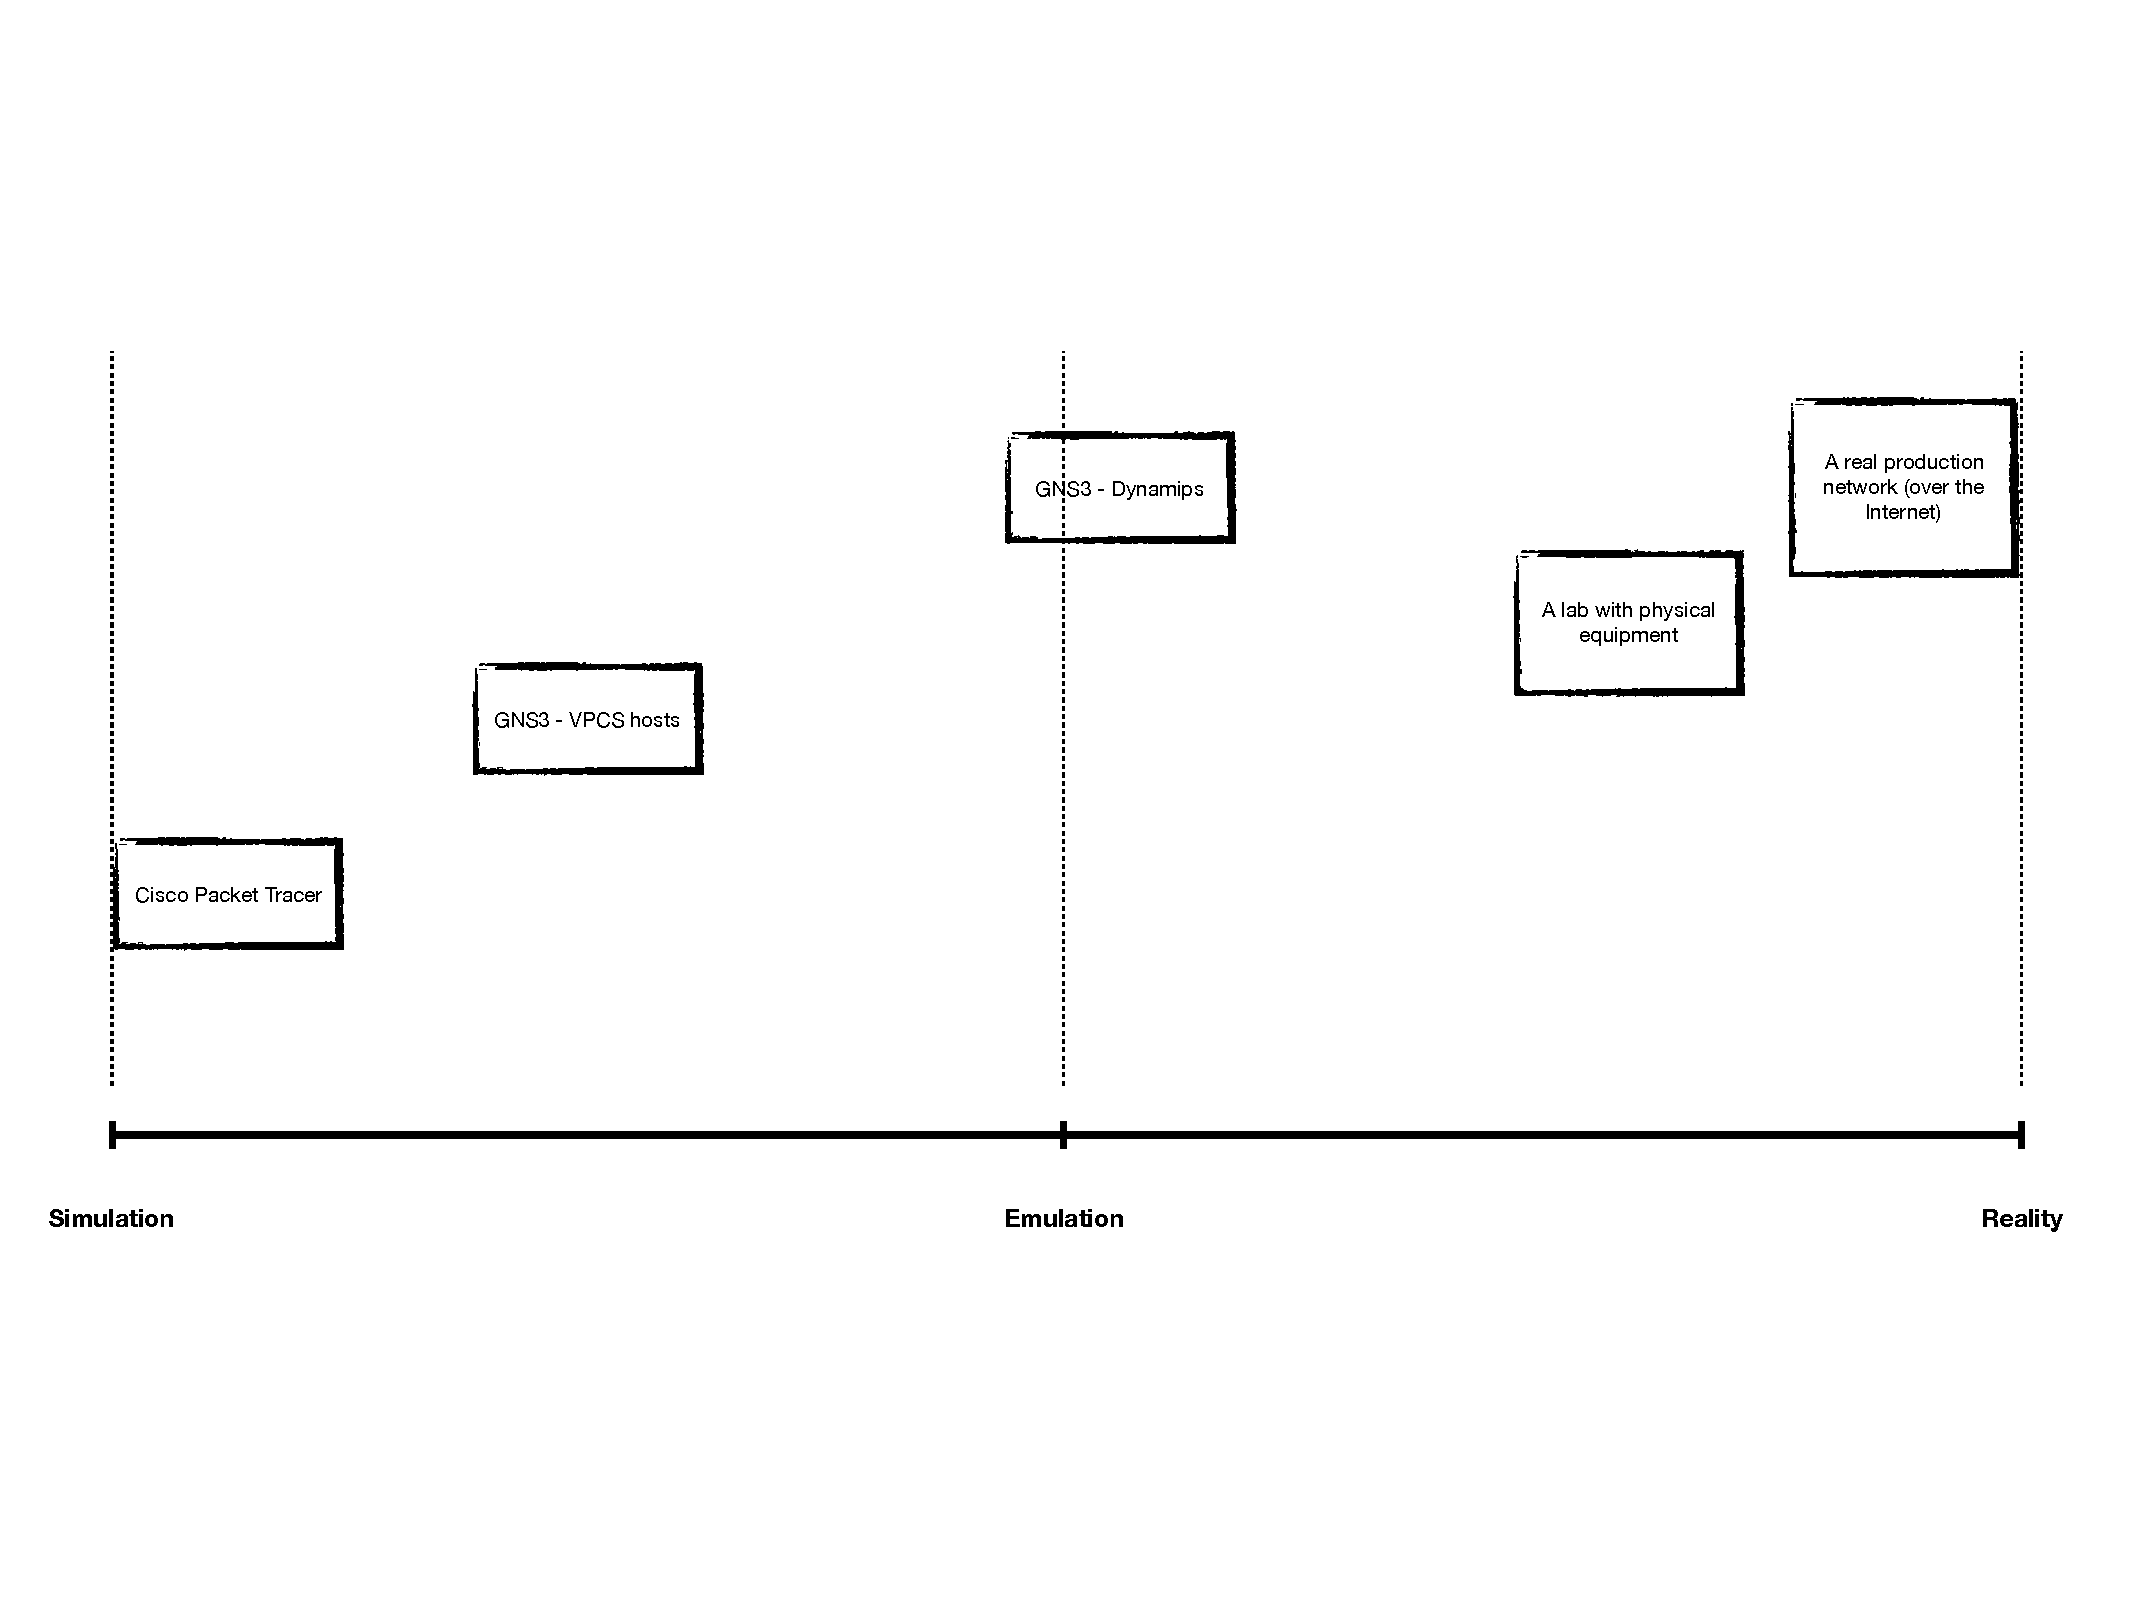
\includegraphics[width=0.8\textwidth]{emulationvsreality}
%   \caption{Simulation vs emulation vs reality}
%   \label{fig:emulationvsreality}
% \end{figure}

Before pointing out the differences between emulators and simulators, it is important to say what both have in common: they are ways of providing students, researches, developers, administrators, or any professional that works with computer networks with an alternative to the real network that is being studied, for convenience and/or cost effectiveness.
However, a lab with network nodes in an education institution is also different from the reality it is trying to model.
%That idea is exposed in the diagram in figure~\ref{fig:emulationvsreality}.

On one end there is reality---in a lab, factors like amount of nodes, physical length of links (and therefore propagation times) can only be \textbf{simulated}, let alone on an solution that is fully software-based, like the emulators described later in this section.
An anecdote like the 500-mile email~\footnote{The case of the 500-mile email~\cite{500mileemail} was an issue described by a systems administrator where e-mails could not be sent to servers further than 500 miles.
The description seemed impossible as e-mail servers (closer) were working, but a hidden configuration---a timeout---rendered a different behavior according to the physical distance between hosts, due to round-trip times.
} could not be reproduced, without simulating an---then---unknown ``flaw,'' in an emulator consisting in virtual machines running the real software and performing the real operations: the cause of the problem was latency.
On the other end there is full simulation, where nothing is real.

In between, complex solutions like GNS3, which is presented in great detail in chapter~\ref{ch:gns3}, can offer a mixture, while being mainly emulators in the sense that it consists in an orchestrated set of processes running the real code, and also allowing to simulate aspects of reality like failures in links and delays.

The reason why emulators are specially interesting and are essentially the motivation (\ref{sec:motivation}) of this work, though, is that giving away the lab room with its switches and cables requires to not lose the flexibility it offers to perform all kind of pedagogical exercises, and ``pure'' simulators do not offer by inherent limitation.

%A network simulator is a computer program (or software package) that implements algorithms corresponding to a \textbf{model} of the reality through software components.
In~\cite{netkit-full}, the article presenting Netkit (a tool studied later in this thesis) and the process that led to its inception, which largely overlaps with the present work, there's an interesting paragraph that explains succinctly the difference between simulation and emulation.
Note that these concepts exist for any kind of \emph{system}, of which any computer system, such as computer networks, are only particular instances (emphasis \textbf{not} present in the original document):
\begin{displayquote}
Simulation aims at computing the behavior of a network based on an abstract model that usually ignores many functional details (e.g., message formats, the need for configurations, and the presence of command line interfaces).
This approach is suited for massive performance-oriented experiments and usually produces accurate event timing information.
Emulation aims at accurately reproducing the behavior of a real network in all its functional details and is usually achieved by exploiting as much as possible the same software (or an open version of it) that would be used on real devices.
Although considerably less efficient than simulation and usually inadequate to reproduce timings observed in real network systems, this approach is very effective to capture the wide range of functionalities and behaviors of a real network, and we believe \emph{it is therefore much more suited for didactics than simulation}.
\end{displayquote}
Simulators like ns-3~\cite{ns3} or the OPNET~\cite{introtoopnet} are discrete event simulators~\cite{netsimoremu}.
They enable, through some interface---such as a graphical one---, designing, testing, analyzing, and observing the expected behavior of protocols, nodes, and links according to several parameters. Therefore, it serves as a way to study protocols used across the stack, and possibly even some application layer components can be ``mimicked''.

Even though the usefulness of these tools cannot be questioned, and some like Cisco Packet Tracer~\footnote{\url{https://www.netacad.com/courses/packet-tracer/introduction-packet-tracer}}, also a discrete event simulator~\cite{evaluatingnetsimmethodologicapproach}, are very widely used in the training of professionals in the networks administration and engineering fields~\cite{rolepackettracer}, it is crucial to point out as the distinctive characteristic of simulators, as defined here, the fact that those applications constitute a ``closed'' universe in the sense of only \emph{simulating} events that change the status of internal data structures, but do not implement a real stack of protocols, where every operation that should be performed is, in fact, performed. % TODO this is super "Portuguese in English". Improve

In other words: a network simulator is a black box for the outside, with a set of available inspection and state alteration operations---i.e. that provides the ability to see some aspects of the simulated system and perform some finite set of changes to the simulated environment.
% However, as long as the \emph{implemented} cause-effect behaviors for that set of operations \emph{is coherent} to their real-world counterparts, any kind of ``shortcuts'' inside can be taken.

On the other hand, the definition for an emulator can, therefore, pretty much be inferred from the simulator as its ``complementary.''
Software computer network emulators are solutions that allow, without resorting to the usage of physical equipment (even though sometimes allow for it, if desired) prototyping networks for analysis and study of underlying mechanisms, investigation, and development of new protocols and solutions, etc., thanks to an array of techniques that can span from virtualization and containerization, hardware architecture emulation, and leveraging operating system functionality in multi-process environments.

Unlike the simulators, described earlier, the fact of the traffic being real (at least from a logical standpoint) and that is possible to ``glue'' emulated interfaces with any kind of physical ones detected by the host operating system, offers the possibility of mixing emulated topologies with real topologies, cloud machines, etc.
Besides, since the computational nodes (hosts in the emulated topologies) are in, fact, ``generic'' hosts (nowadays, usually VMs or containers), running real software, the limit in terms of what it is possible to configure, parameterize, implement, or test, for any stack level (from the link to the application layer) is virtually nonexistent.

% end of section leavingemulationandsimulation


Providing a precise definition, or ``definition framework,'' for distinguishing simulators from emulators and why \emph{emulation} (as opposed to \emph{simulation}) is the focus of this dissertation is paramount.
In the literature, Wikipedia, or common dictionaries, there are contradictory definitions, overlapping concepts, and, in general, a vague distinction between the two is presented~\cite{netsimoremu}. % TODO find and insert citations
That is why, rather than universally establishing what an emulator and a simulator are, it is intended that when, throughout this text, software package $A$ is an emulator and $B$ is a simulator in this or that sense, the reader can know without ambiguity what is meant.

% \begin{figure}
%   \centering
%   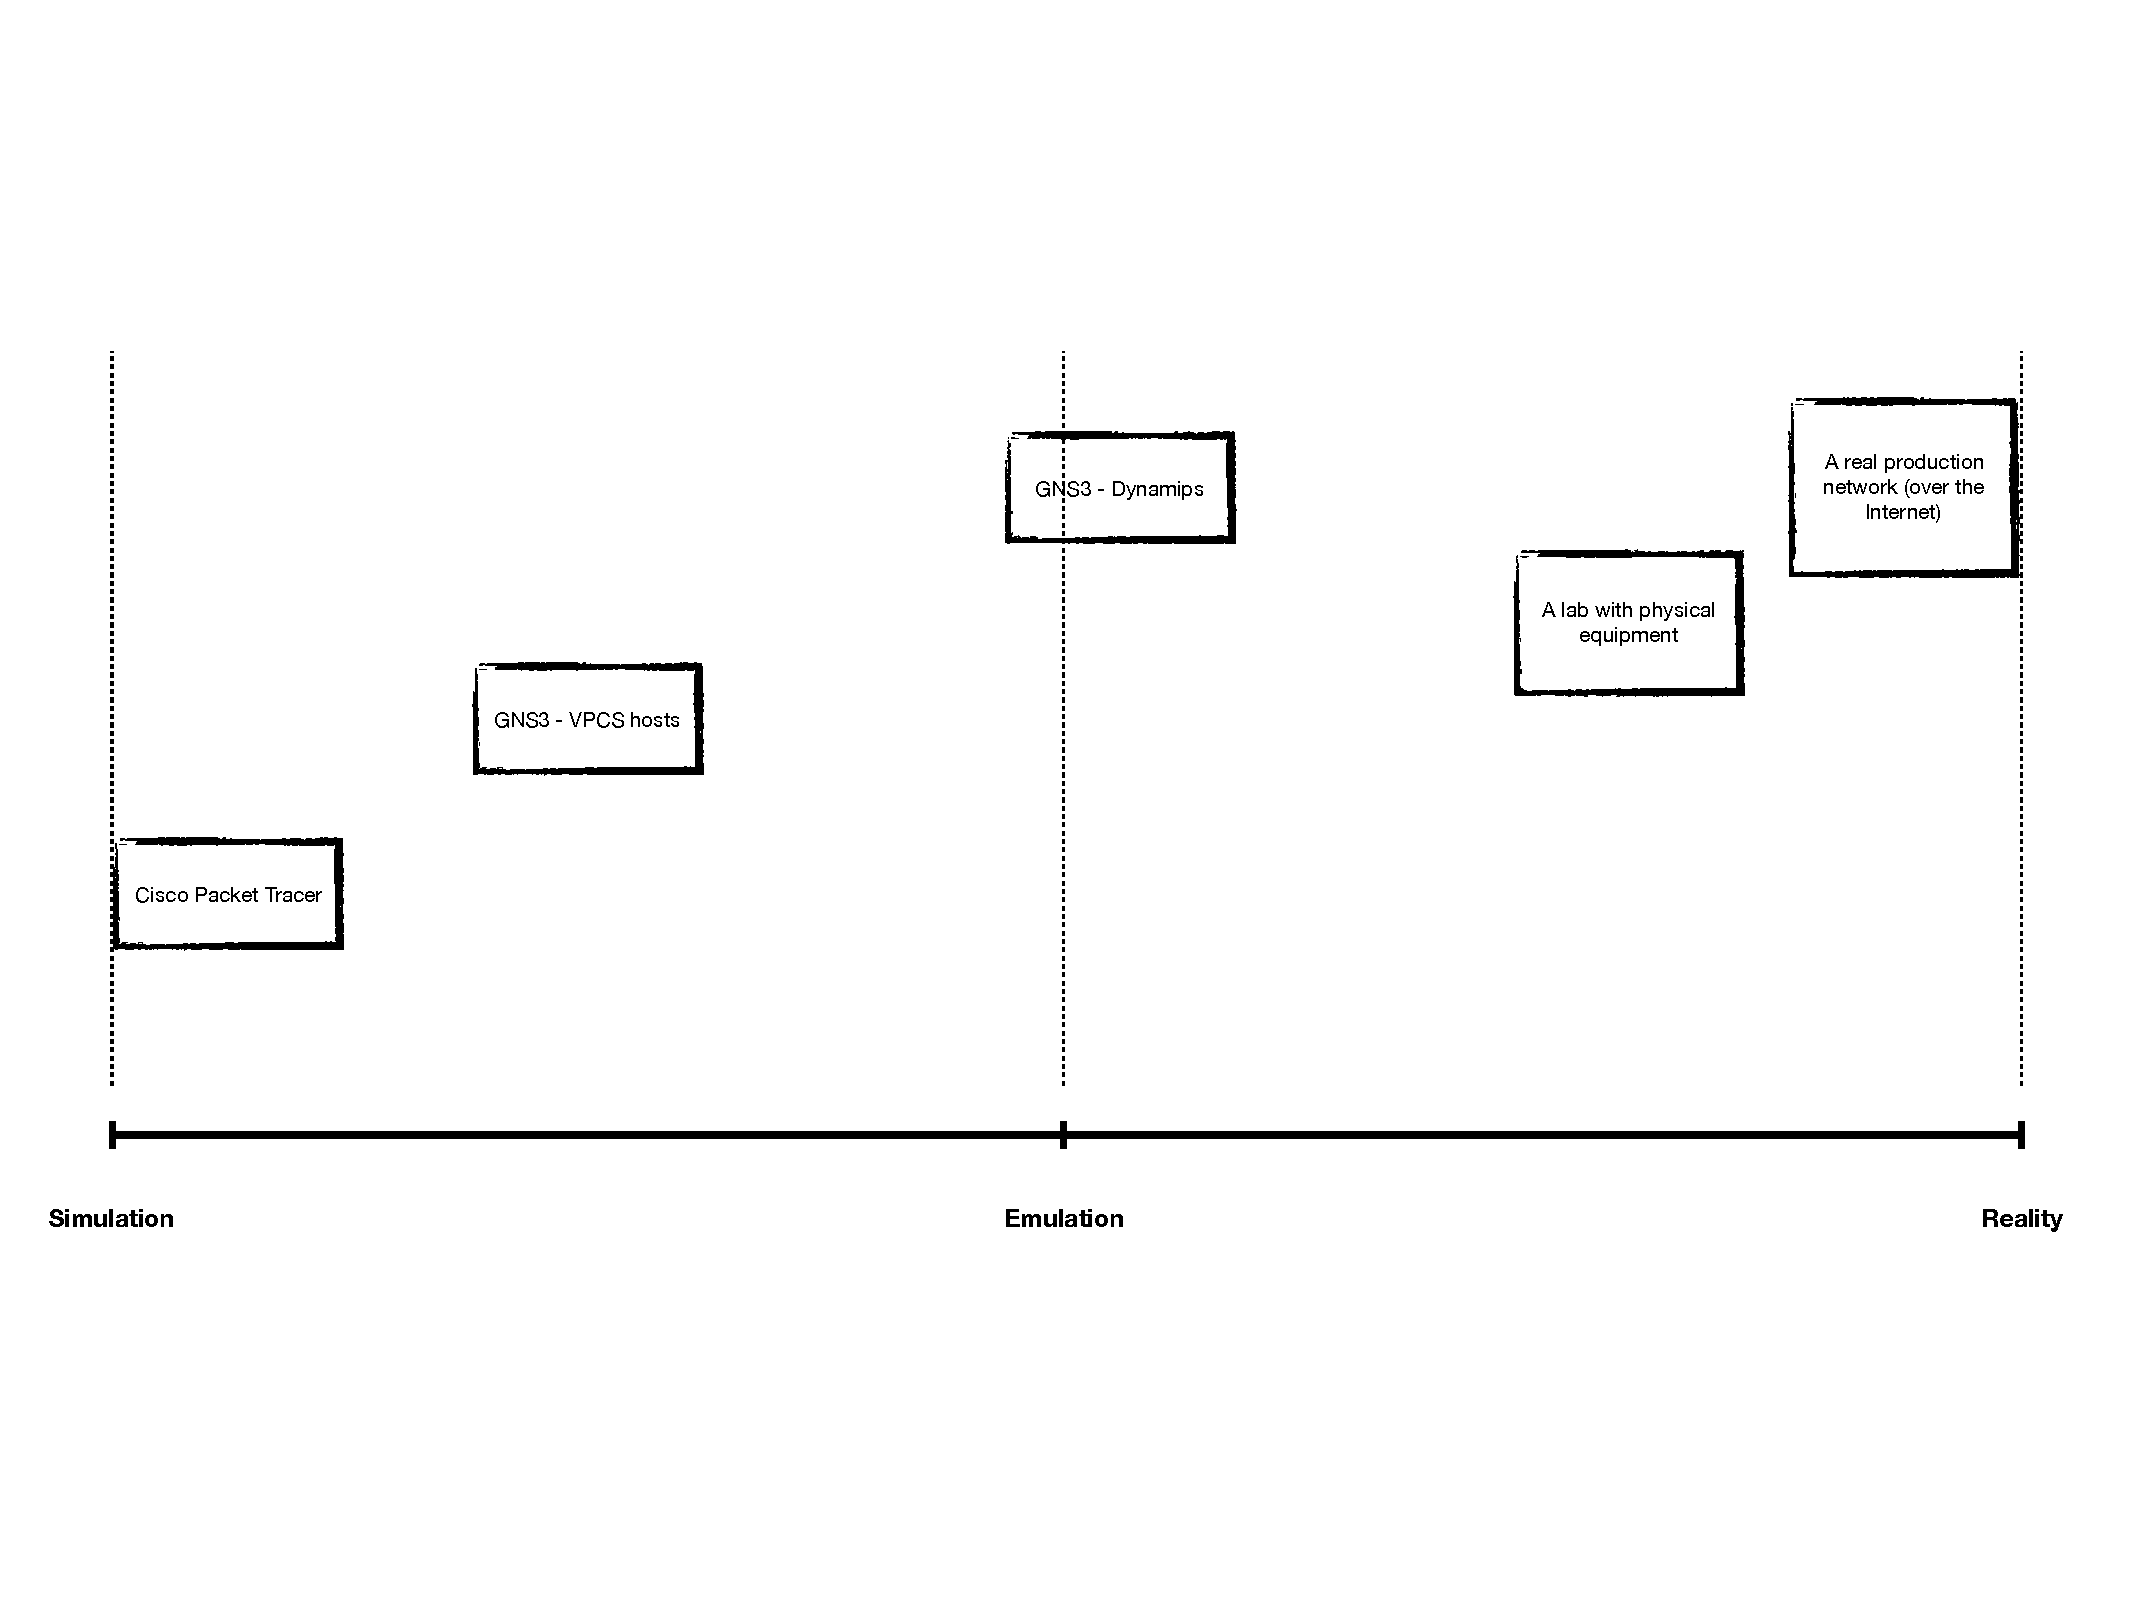
\includegraphics[width=0.8\textwidth]{emulationvsreality}
%   \caption{Simulation vs emulation vs reality}
%   \label{fig:emulationvsreality}
% \end{figure}

Before pointing out the differences between emulators and simulators, it is important to say what both have in common: they are ways of providing students, researches, developers, administrators, or any professional that works with computer networks with an alternative to the real network that is being studied, for convenience and/or cost effectiveness.
However, a lab with network nodes in an education institution is also different from the reality it is trying to model.
%That idea is exposed in the diagram in figure~\ref{fig:emulationvsreality}.

On one end there is reality---in a lab, factors like amount of nodes, physical length of links (and therefore propagation times) can only be \textbf{simulated}, let alone on an solution that is fully software-based, like the emulators described later in this section.
An anecdote like the 500-mile email~\footnote{The case of the 500-mile email~\cite{500mileemail} was an issue described by a systems administrator where e-mails could not be sent to servers further than 500 miles.
The description seemed impossible as e-mail servers (closer) were working, but a hidden configuration---a timeout---rendered a different behavior according to the physical distance between hosts, due to round-trip times.
} could not be reproduced, without simulating an---then---unknown ``flaw,'' in an emulator consisting in virtual machines running the real software and performing the real operations: the cause of the problem was latency.
On the other end there is full simulation, where nothing is real.

In between, complex solutions like GNS3, which is presented in great detail in chapter~\ref{ch:gns3}, can offer a mixture, while being mainly emulators in the sense that it consists in an orchestrated set of processes running the real code, and also allowing to simulate aspects of reality like failures in links and delays.

The reason why emulators are specially interesting and are essentially the motivation (\ref{sec:motivation}) of this work, though, is that giving away the lab room with its switches and cables requires to not lose the flexibility it offers to perform all kind of pedagogical exercises, and ``pure'' simulators do not offer by inherent limitation.

%A network simulator is a computer program (or software package) that implements algorithms corresponding to a \textbf{model} of the reality through software components.
In~\cite{netkit-full}, the article presenting Netkit (a tool studied later in this thesis) and the process that led to its inception, which largely overlaps with the present work, there's an interesting paragraph that explains succinctly the difference between simulation and emulation.
Note that these concepts exist for any kind of \emph{system}, of which any computer system, such as computer networks, are only particular instances:
\begin{displayquote}
Simulation aims at computing the behavior of a network based on an abstract model that usually ignores many functional details (e.g., message formats, the need for configurations, and the presence of command line interfaces).
This approach is suited for massive performance-oriented experiments and usually produces accurate event timing information.
Emulation aims at accurately reproducing the behavior of a real network in all its functional details and is usually achieved by exploiting as much as possible the same software (or an open version of it) that would be used on real devices.
Although considerably less efficient than simulation and usually inadequate to reproduce timings observed in real network systems, this approach is very effective to capture the wide range of functionalities and behaviors of a real network, and we believe it is therefore much more suited for didactics than simulation.
\end{displayquote}
Simulators like ns-3~\cite{ns3} or the OPNET~\cite{introtoopnet} are discrete event simulators~\cite{netsimoremu}.
They enable, through some interface---such as a graphical one---, designing, testing, analyzing, and observing the expected behavior of protocols, nodes, and links according to several parameters. Therefore, it serves as a way to study protocols used across the stack, and possibly even some application layer components can be ``mimicked''.

Even though the usefulness of these tools cannot be questioned, and some like Cisco Packet Tracer~\footnote{\url{https://www.netacad.com/courses/packet-tracer/introduction-packet-tracer}}, also a discrete event simulator~\cite{evaluatingnetsimmethodologicapproach}, are very widely used in the training of professionals in the networks administration and engineering fields~\cite{rolepackettracer}, it is crucial to point out as the distinctive characteristic of simulators, as defined here, the fact that those applications constitute a ``closed'' universe in the sense of only \emph{simulating} events that change the status of internal data structures, but do not implement a real stack of protocols, where every operation that should be performed is, in fact, performed. % TODO this is super "Portuguese in English". Improve

In other words: a network simulator is a black box for the outside, with a set of available inspection and state alteration operations---i.e. that provides the ability to see some aspects of the simulated system and perform some finite set of changes to the simulated environment.
% However, as long as the \emph{implemented} cause-effect behaviors for that set of operations \emph{is coherent} to their real-world counterparts, any kind of ``shortcuts'' inside can be taken.

On the other hand, the definition for an emulator can, therefore, pretty much be inferred from the simulator as its ``complementary.''
Software computer network emulators are solutions that allow, without resorting to the usage of physical equipment (even though sometimes allow for it, if desired) prototyping networks for analysis and study of underlying mechanisms, investigation, and development of new protocols and solutions, etc., thanks to an array of techniques that can span from virtualization and containerization, hardware architecture emulation, and leveraging operating system functionality in multi-process environments.

Unlike the simulators, described earlier, the fact of the traffic being real (at least from a logical standpoint) and that is possible to ``glue'' emulated interfaces with any kind of physical ones detected by the host operating system, offers the possibility of mixing emulated topologies with real topologies, cloud machines, etc.
Besides, since the computational nodes (hosts in the emulated topologies) are in, fact, ``generic'' hosts (nowadays, usually VMs or containers), running real software, the limit in terms of what it is possible to configure, parameterize, implement, or test, for any stack level (from the link to the application layer) is virtually nonexistent.

% \section{Notable simulators}
% \label{sec:notablsimulators}

% Packet Tracer, Boson NetSim, ns-3...

% \section{Notable emulators}
% \label{sec:notablemulators}

% \subsection{GNS3}
% \label{subsec:relworkgns3}

% \subsubsection{Usage of GNS3 in education}
% \label{subsubsec:relgns3usageedu}

% There is already some published work about using GNS3 in education institutions.
% Usually, though, the experiments and comparisons are made against other ``graphical simulators''---instead of emulators---, since those are the software tools that, from a high-level perspective are equivalent, even if the functional possibilities and implementations are completely different, if not opposite.

% A brief comparison with Boson NetSim and Packet Tracer, two graphical simulators, is presented in~\cite{virtlabgnsvmware}, where the authors explain a way to use VMware Workstation VMs on a desktop to ``emulate'' end hosts on GNS3's virtual topologies, and using applications on those VMs which communicate with each other over the emulated links.

% In~\cite{automaticnetconfiggns}, the authors, two Professors from the Polytechnic Institute of Leiria, Portugal, dive into ways to automate GNS3 topology configurations, which, as will be seen in chapter~\ref{ch:gns3}, can be a major issue. % TODO

% The usefulness for distance learning is also explored, for example, in~\cite{networkvirtwithgns}.

% \subsection{Kathara}
% \label{subsec:relworkkathara}

% \subsection{CORE}
% \label{subsec:relworkcore}

% \subsection{Mininet}
% \label{subsec:relworkmininet}

% \section{Usage of simulators and emulators in teaching}
% \label{sec:simemulusage}

% end of chapter

  % !TEX root = ../Thesis.tex
% !TEX spellcheck = en-US

\chapter{Examples of emulators}
\label{ch:examplesofemulators}

% \section{Section 1}
% \label{sec:relsec1}

% \section{Section 2}
% \label{sec:relsec2}

% end of chapter

  % !TEX root = ../Thesis.tex
% !TEX spellcheck = en-US

\chapter{GNS3}
\label{ch:gns3}

% GNS3, whose original name was ``Graphical Network Simulator-3,'' is a software project, comprising several distinct components and, despite the ``simulator'' in its name, it falls under the category of emulators (cf.~\ref{sec:emulationsimulation}): its operation runs real code accross all the layers of the stack. % TODO try to (either with a source, or speculating) relate the name with ns-3
% TODO also: cite the source for the name
% By ``as a whole,'' it is meant that, as shall be seen later, although some of its components, like the Dynamips program, are emulators in a very strict sense---i.e. its purpose is to run real machine code on a different hardware architecture (than its native one)---, it differentiates itself, on a high-level perspective, from a simulator which is a program designed to execute a mathematical model, processing modeled events as internal data-structures with a collection of preset algorithms that somehow mimic (a part of) the reality. % TODO: delete?

% Note that a necessary step towards the goal of this this thesis is to systematize a technical description of the architecture and functional underpinnings of the GNS3 system.
% How does it interact with the hardware and software it is running in, how much resources does it take to work with GNS3 according to the ``mode'' it is running in, etc., as that is an aspect that is yet to be further explored for, at least, the following reasons:  % TODO improve the writing how is etc written in Engilsh?
% on the one hand, the consulted academic material (i.e. research papers, mostly) is very brief and omissive in regards to the design, architecture and implementation of GNS3, and so is the official website and documentation; on the other hand, many interesting details are in the ``paraofficial'' videos available via YouTube, mostly by David Bombal,\footnote{\url{https://www.youtube.com/channel/UCP7WmQ_U4GB3K51Od9QvM0w}} namely a comprehensive overview of the architecture (compared with the functionality) of GNS3 by its creator, Jeremy Grossmann, and essentially are not anywhere else, at least from authoritative sources. % TODO same as the previous "sentence". Cite the videos (how and which ones?)

% TODO add a figure (a screen shot) showing the "official" submitter of GNS3 videos (and maybe the channel and/or links from the gns3 official website)

% end of intro

% The first section of this chapter explains the motivation behind the creation of GNS3, as that fact determines implementation and functional aspects of this piece of software.
This chapter consists in a detailed analysis and study of one of the two examples given in chapter~\ref{ch:examplesofemulators} which were chosen to be looked into more depth and, later, compared against each other---the GNS3 emulator.
First, two sections present GNS3 from a more technical angle:
  \begin{enumerate*}[label=(\roman*), itemjoin={{, }}, itemjoin*={{, and }}]
  \item a description of the architecture and the main design characteristics of GNS3 are explained, giving a good overview of the kind of setup it needs, and in what kind of environments it can be executed and inherent scalability features
  \item the implementation solutions chosen by GNS3's developers to provide its high-level functionality.
  \end{enumerate*}
Then, the chapter finishes by presenting a case-study that directly addresses the problem which motivates this thesis and describes how GNS3 offers solutions for that problem, and then performance and resource consumption considerations, result of the observation done mainly during the performance of the case-study, are exposed in a systematic way.

% Section "Architecture and building blocks"
\section{Architecture and building blocks}
\label{sec:gns3architecture}

A good written, comprehensive description of the GNS3 architecture and technical details is lacking.
There is a page, on the online developers-oriented documentation~\cite{gns3devarch}, which presents a very simple diagaram, that is reproduced\footnote{Dashed strokes are added by the author of the thesis to provide extra information} on figure~\ref{fig:gns3-docs-arch}.
Even the two published books that exist on the project~\cite{gns3netsimguide,thebookofgns3} are omissive or very brief, not allowing for gaining an in-depth knowledge, necessary to understand the possible issues of performance, resource consumption, scalability, and functional limitations that GNS3 may suffer from.
Going from the simple diagram that was mentioned towards a more complete reference is one of this thesis' efforts.

To accomplish such effort, a precious resource has been the ``paraofficial'' videos available via YouTube, mostly by David Bombal, an instructor and close collaborator of the GNS3 organization, namely a comprehensive overview of the architecture (compared with the functionality) of GNS3 by its creator, Jeremy Grossmann~\cite{ytgns3arch22}, and essentially are not anywhere else, at least from authoritative sources. % TODO do nothing with \footnote{\url{https://www.youtube.com/channel/UCP7WmQ_U4GB3K51Od9QvM0w}} ?

% Figure fig:gns3-docs-arch
\begin{figure}
  \centering
  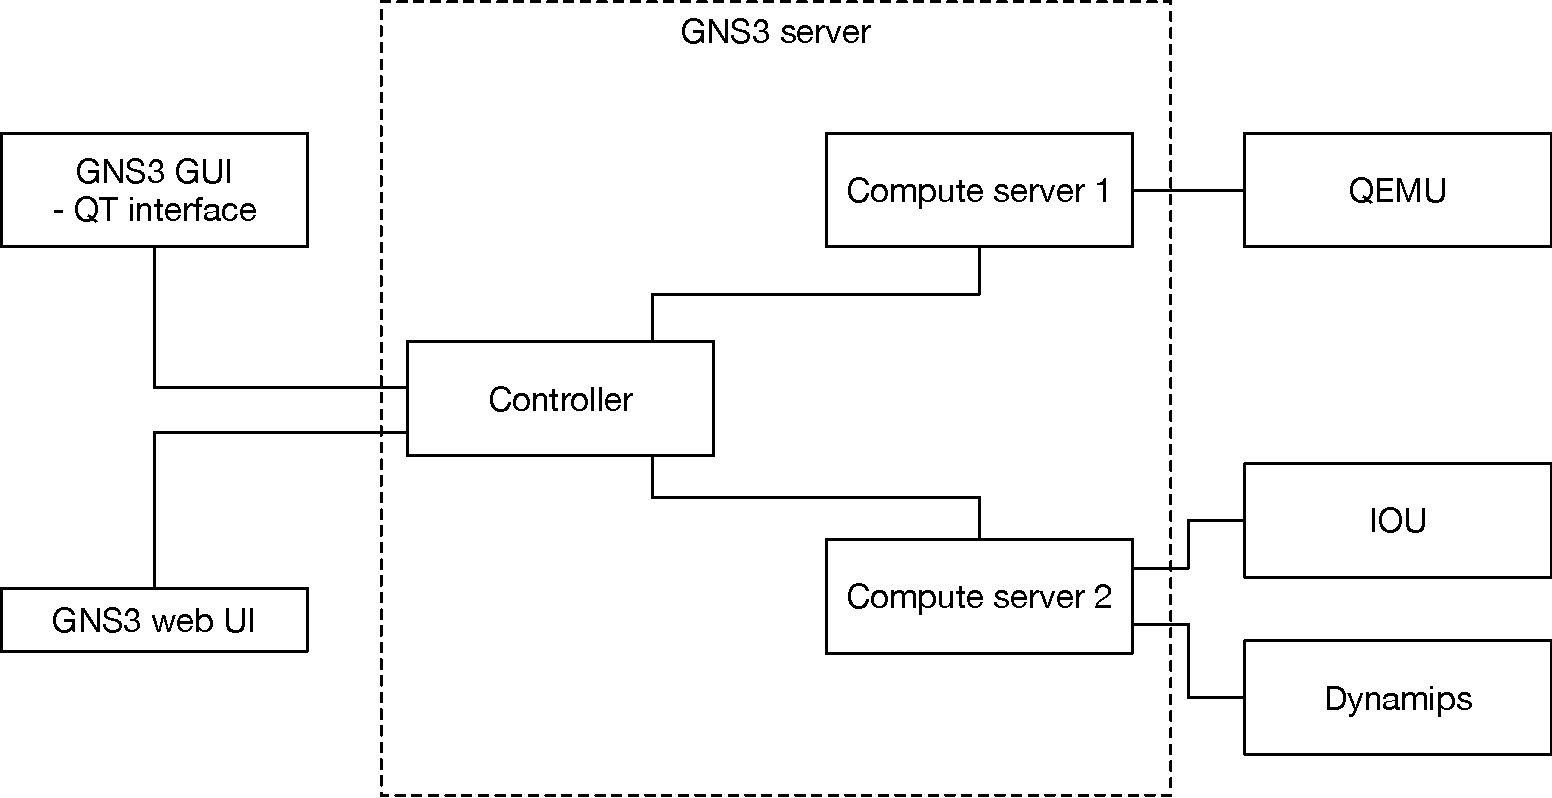
\includegraphics[width=0.8\textwidth]{gns3-docs-arch}
  \caption{The architecture of GNS3 (adapted from the official documentation)}
  \label{fig:gns3-docs-arch}
\end{figure}


\subsection{The simple client-server perspective}
\label{subsec:gns3clientserver}

GNS3 works, first and foremost, as a client-server application.
The standard installation for desktop provides all the necessary to components to fully(-ish) work on that physical machine, but the client doesn't have to be, and in many real scenarios isn't, running on the same host as the server.
However, in fact, a \textbf{topology}---the name GNS3 gives to its ``projects,'' which comprises of nodes (emulated/virtualized routers, switches, SDN-controllers, virtual PCs, interfaces for hardware network connections)---can be running in different machines, even on the ``backend'' side itself, as will be seen.

The \textbf{GNS3 server} exposes a public \acrshort{rest} \acrshort{api}, documented in~\cite{gns3devarch}, which is the way any client edits the opened topology or performs actions on the nodes contained therein, or in the GNS3 running environment.
GNS3 server, described more thoroughly afterwards, is the brains and central point of topology opened and in-execution.
It has first-hand knowledge of events that occur in the nodes, their status, their interfaces' status, and communicates with the several means existing to actually provide the \emph{emulation} for each specific node.
All of this will be analyzed and explained posteriorly.
For now, it suffices to see it as a central point, accessible by any number of clients, of a running topology.

To interact with the system, by editing a topology, or performing actions on nodes---all the items in the topology, which can be connected via links---, one or more users simultaneously can utilize a graphical client. The \textbf{GNS3 GUI}, part of a standard installation on any desktop operating system, namely macOS, a desktop Linux distribution (official repositories for Ubuntu exist), or Windows,\footnote{\url{https://gns3.com/software/download}} is a cross-platform application developed using the Qt graphical toolkit~\cite{qttoolkit}.
They may also use a web UI (somewhat limited yet), or any tool, user-driven or automatic, programmed to send requests and receive responses according to the aforementioned REST specification.
The official clients, bundled with the GNS3 installation packages for desktop environments, GNS3 GUI and the official web UI, show an in-real-time view of the topology---e.g. the status of virtual network interfaces, or changes made by other client---thanks to WebSockets server-to-client calls~\cite{ytgns3arch22}. % TODO link WS to the glossary, when definition is available

% Figure fig:gns3-2hosts2routers-macOS
\begin{figure}
  \centering
  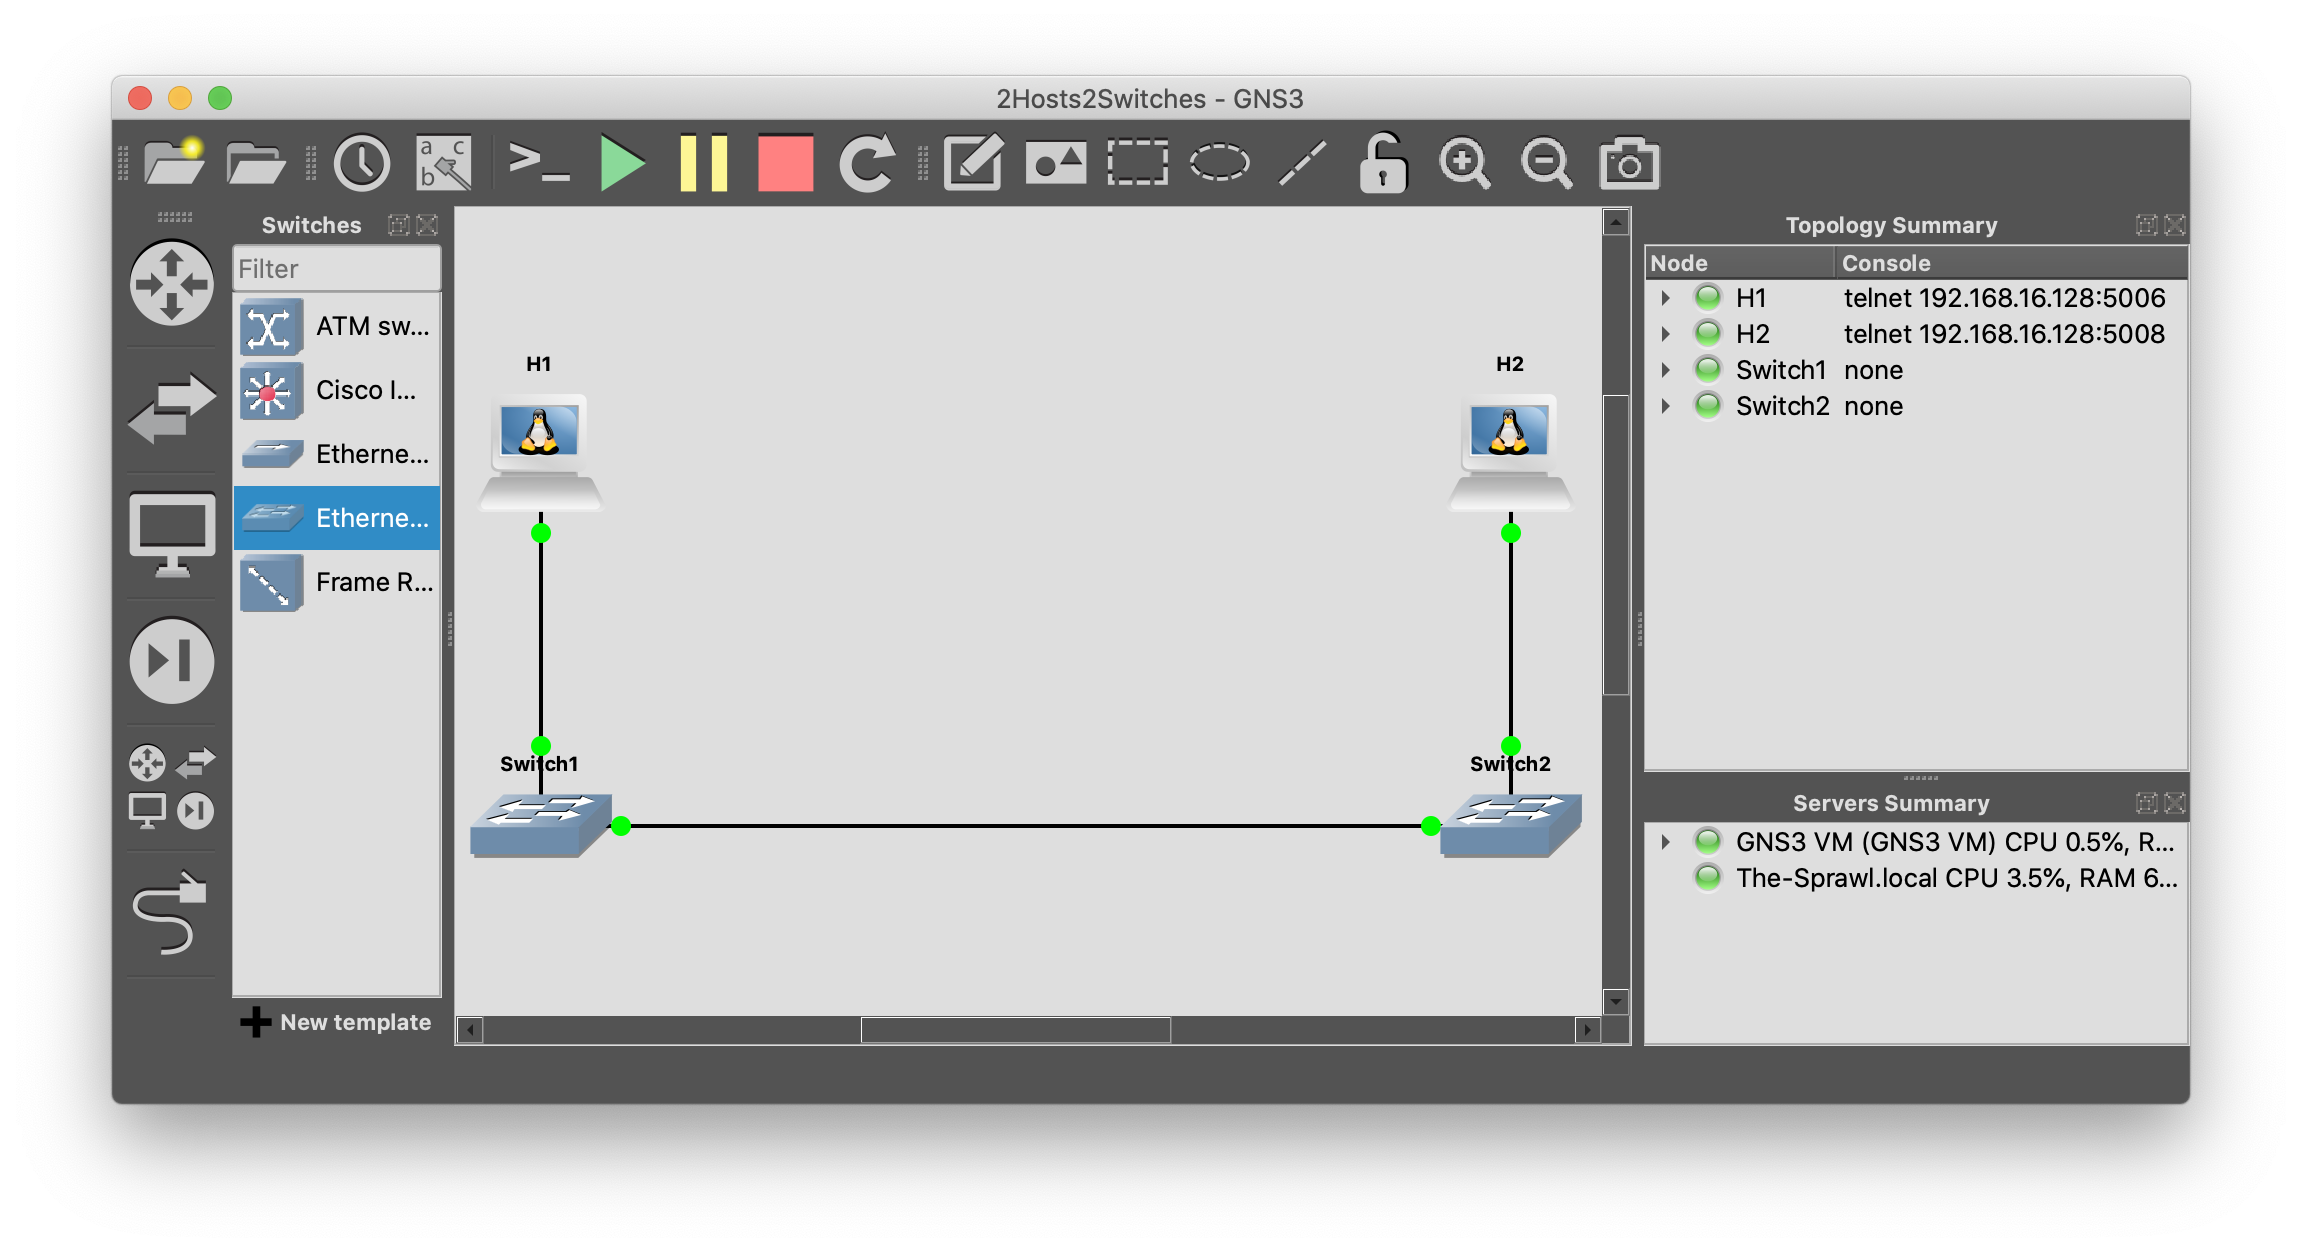
\includegraphics[width=0.8\textwidth]{gns3-2hosts2routers-macOS}
  \caption{Simple topology with only two switches and two virtual PCs as seen on the GUI in macOS}
  \label{fig:gns3-2hosts2routers-macOS}
\end{figure}


\subsection{The GNS3 server---distributed}
\label{subsec:gns3serverindetail}

The GNS3 server is a program with a code-base independent from other parts of the project.
The software package \texttt{gns3-server} can be obtained from official repositories for Linux systems to install it on servers without video interface, with users running some of the already mentioned clients in their laptops or desktop computers.
It is also possible to obtain a VMware ESXi image to directly spin-up a GNS3 server ready machine on an virtualized infrastructure.

The same program behaves as two different roles, both of which are necessary to get the GNS3 system working.

\begin{itemize}
	\item The \textbf{controller node}, or just ``controller,'' of which there can only be one instance per running topology, and is ``[its] decision point'' (Jeremy Grossmann's words); the process responsible by fulfilling the client's requests and postback real-time information to them and know the hosts where nodes may be running.
	\item The \textbf{compute node}, referred to simply as ``compute'' too, which, for one running topology, can be running $N$ times, one per each machine (physical or virtual) taking care of emulating one or more topology nodes (again: switches, routers, etc.).
	It is this separation and the ability to have multiple compute nodes that allows GNS3 to be configured in a way that can serve arbitrarily large topologies, since the cost in resources of an increasing number of ``live'' nodes can be balanced among an also increasing number of servers running a compute.
\end{itemize}

When the server is running on a single host, one \texttt{gns3-server} program instance (i.e. process) performs both roles, controller and compute.
However, when the server is distributed across one or more machines, communication between the controller and the computes on other hosts happens through a REST API.
That API is a private or internal one, unlike the one for client-server, and there isn't a programmer's manual for developing with it.
Only the (single) controller is supposed to communicate with each process acting as compute.

% end of section gns3architecture


% Section "Brining topologies to life---emulating nodes and links"
\section{Bringing topologies to life---emulating nodes and links}
\label{sec:gns3emulating}

On section~\ref{sec:gns3architecture}, an overview of the way GNS3 is organized and runs in a distributed fashion was provided.
However, a crucial part is missing: how can the compute nodes, coordinated by the controller, which in turn is commanded by one or more clients, give life to the nodes that are put into a topology, seen in the GUI represented by their respective icons.
And also what mechanism is used to pass along the traffic transmited, received, switched, or any other action a possible node does while running via the links connected to the interfaces.

\subsection{Appliances}
\label{subsec:gns3appliances}

Each element of the set of possible nodes to be added to a topology on someone's GNS3 installation and setup is called an \textbf{appliance}.
GNS3 has a templating system for creating appliances, apart from the ones that come ``pre-installed.''
Many templates are immediately accessible from the GUI.
These allow to prepare the GNS3 setup to be able to put in topologies certain nodes that it supports well but include components which cannot be distributed together with GNS3 for legal reasons or are simply too heavy and/or niche-oriented for bundling it by default to be worth it.
That is the case for commercial routers and switches that can be emulated in GNS3.

An example can be given with the better documented case of GNS3: setting up topologies using Cisco's layer 2 and~3 routers via the vendor's proprietary IOSv images described later in more detail later.
Since, to boot these virtual devices, images distributed only by Cisco, under specific conditions and exclusively to users having certain licenses, are required, the user must create an appliance from the template in each of their GNS3 installation, uploading the IOSv L2 or L3 image.
However, thanks to the templates, after providing the missing component, the emulator already knows how to boot the images and orchestrate together with the rest of the rest of the software's functionality.

% When, for example, a user intends to carry out one of the most common use-cases for GNS3---making a topology with Cisco IOSv nodes, which needs Cisco's official disk images---that appliance is not ready to be used on the appliances dock on the GUI.
% Instead they can easily access the template for it, which provides almost all inner parametrization and is a ``placeholder'' for that kind of node, provide the corresponding virtual disk image, which they should have downloaded and have licensed, and the client application takes care of uploading it to the server (local or remote), rendering the appliance available to be dragged-and-dropped into the topology canvas.

The panel (dubbed ``dock'' in GNS3 parlance) where the available devices are shown is depicted in figure~\ref{fig:gns3-appliances-dock}.
In this case, only the Cisco IOSvL2 switch and the Ubuntu Docker Guest were added after the base installation.
The other available nodes are stock.
Figure~\ref{fig:gns3-appliances-from-server-routers} shows the dialog where a partial list of available appliance templates is ready to be selected.

% Figure fig:gns3-appliances-dock and fig:gns3-appliances-from-server-routers
\begin{figure}
\centering
\begin{minipage}{.4\textwidth}
  \centering
  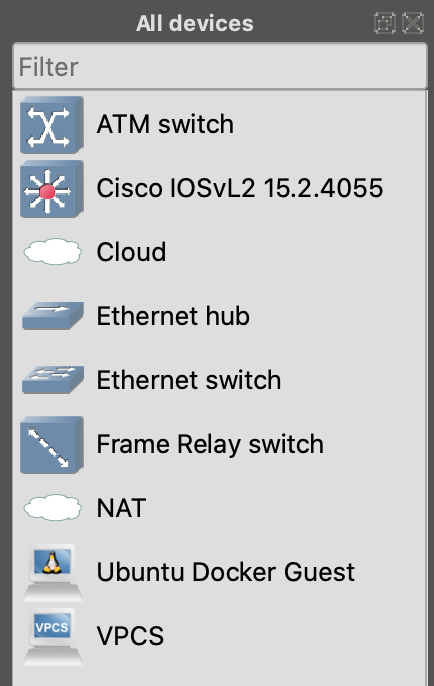
\includegraphics[width=.8\linewidth]{gns3-appliances-dock}
  \captionof{figure}{The appliances dock}
  \label{fig:gns3-appliances-dock}
\end{minipage}%
\begin{minipage}{.6\textwidth}
  \centering
  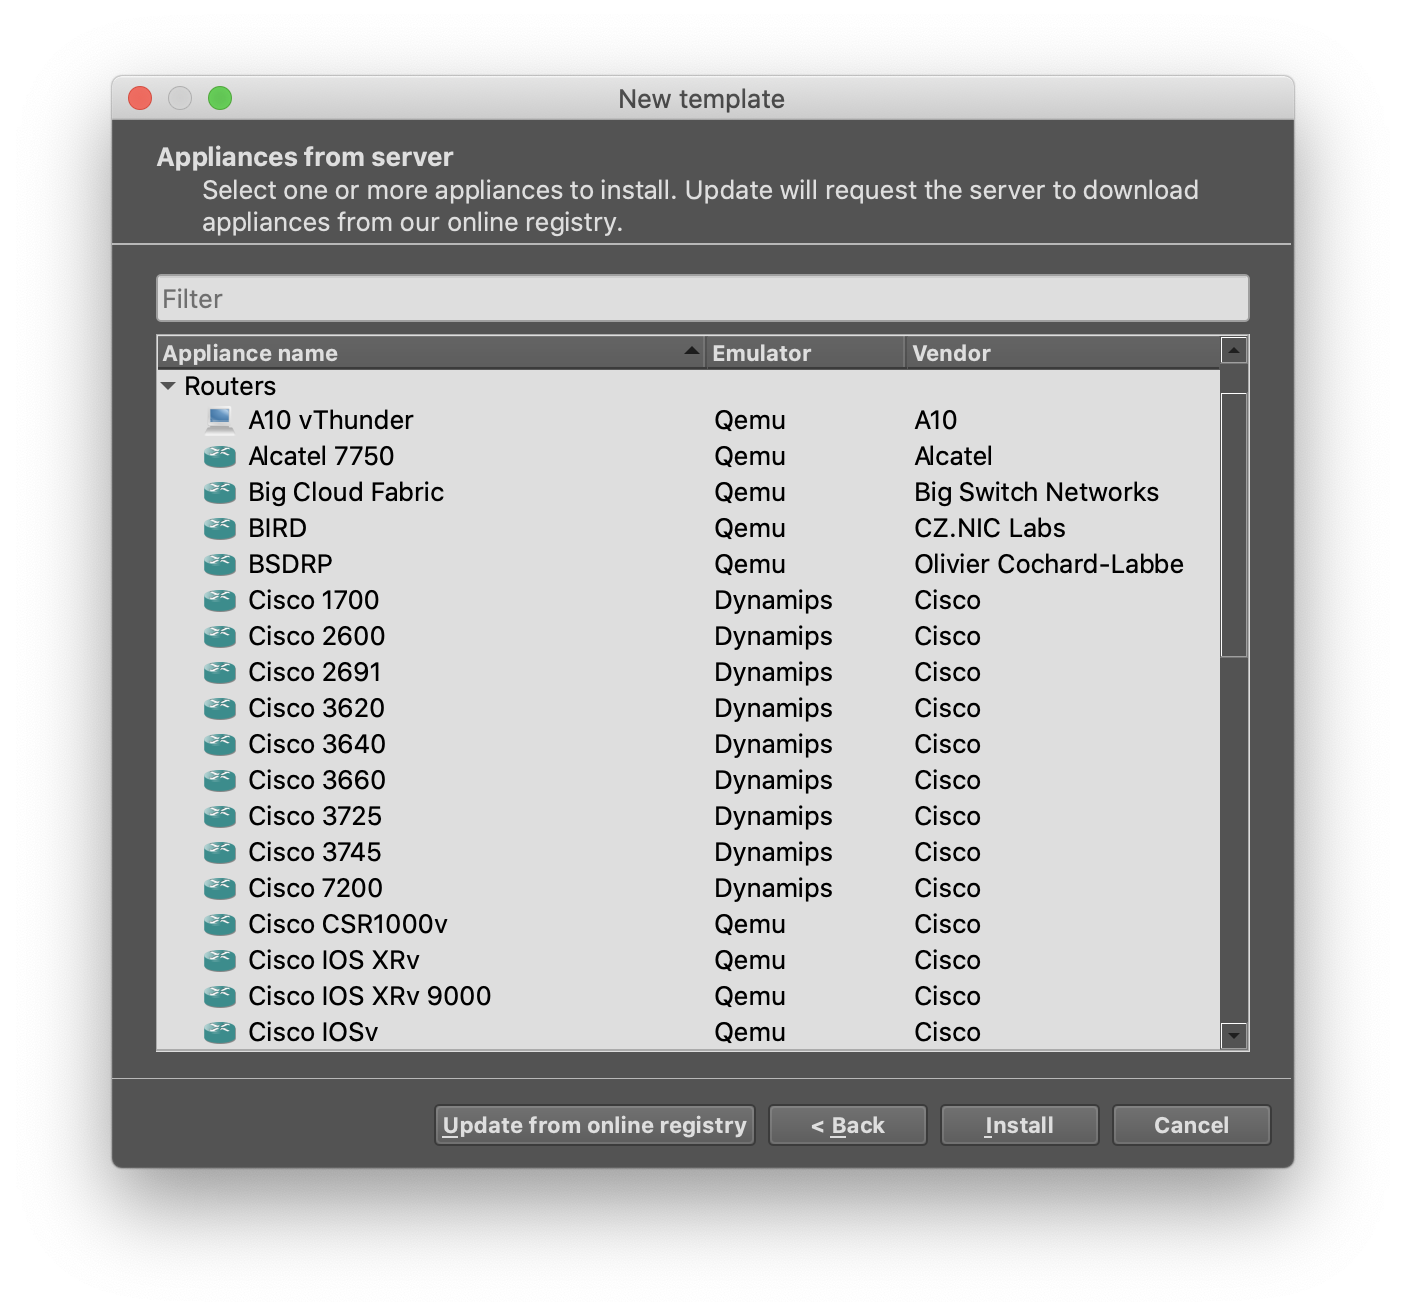
\includegraphics[width=.95\linewidth]{gns3-appliances-from-server-routers}
  \captionof{figure}{Some available router templates}
  \label{fig:gns3-appliances-from-server-routers}
\end{minipage}
\end{figure}


Deliberately, \emph{commercial} vendors of hardware, whose emulation is supported by GNS3, other than Cisco are excluded from this case-study for the following reasons:

\begin{enumerate}
  \item There isn't as near as many documentation and references in the literature, the web, or academic material for it as there is for Cisco.
  \item To narrow the scope of the investigation and this document, as the (again, commercial) network gear in laboratory used for the case study, FCT/NOVA's, is exclusively Cisco.
\end{enumerate}

Thus, this section is not intended to be exhaustive, or even less complete, in the sense of covering all the means GNS3 supplies out-of-the-box to emulate possible nodes in topologies.

\subsection{Dynamips and legacy Cisco routers}
\label{subsec:gns3dynamipslegacy}

GNS3 was initially built to leverage the Dynamips emulator~\cite{thebookofgns3}.
It consists of a pure hardware emulator for MIPS processors geared towards full-compatibility with a series of Cisco (now legacy) router hardware models, namely the 1700, 2600, 3600, 3700, and 7200 series. % TODO add 'MIPS' to gls
Not only it the emulator is able to execute MIPS machine-level instructions, it also is able to boot real, uncompressed images for the real hardware and provide virtual interfaces and slots for modules corresponding to those in the physical counterparts.

Dynamips does not support Cisco Catalyst layer-2 switches, only the aforementioned layer-3 modular routers.
All it offers for switching capabilities is, for some models, the ability to insert a module, called EtherSwitch, which provides 16 switched ports to the routers, and allows for \emph{some} experiments with the switching capabilities (VLANs, STP) to be made.
However, \cite{thebookofgns3}, which has a lengthy reference on using Dynamips, its advantages and disadvantages is clear in stating that it isn't without its limitations, which comprehensively listed in this reference.

In a video published in the already mentioned semi-official GNS3 YouTube channel, the software's creator Jeremy Grossmann clearly states that Dynamips is not recommended for production these days, since, as will be seen later, more modern and maintainable solutions exist. At the same time, the GNS3 creator and lead developer also states that there are not plans to remove Dynamips support in upcoming versions~\cite{ytdynamipsvpcs}.

That is not say that, if no ``advanced'' features are intended, Dynamips, whose processes are extremely light compared to most of the alternatives, isn't the right solution, in the user or institution has access to licensed legacy IOS images. % TODO add ref to the performance part

\subsection{QEMU and Cisco IOSv}
\label{subsec:gns3ciscoiosv}

Another way to have Cisco gear inside a topology is using Cisco IOSv images, provided by the vendor itself as part of having access to their proprietary Virtual Internet Routing Lab (VIRL)~\cite{ciscovirl}.
IOSv, which concretely are IOSvL2 and IOSvL3 (standing for layer-2 and layer-3, respectively) are described as ``an implementation of Cisco IOS running as a full virtual machine on a hypervisor''~\cite{ciscoiosvinfo}.

On GNS3 this is accomplished via QEMU, a free and open source, general purpose emulator.
In particular, the way GNS3 uses QEMU is not as an emulator, but as a wrapper for KVM~\cite{whatiskvm}, which ensures extremely good virtualized performance, though naturally limited to the resources of the hypervisor machine:
\begin{displayquote}
Run KVM and Xen virtual machines with near native performance.\footnote{\url{https://www.qemu.org}}
\end{displayquote}

When an appliance for IOSv is added to a GNS3 setup using the template, a virtual disk image is provided and uploaded to the compute node.
It is then used for spinning up VMs with virtual interfaces running the operating system provided in the image. % TODO make this an acr statement

\subsection{Guests and other appliances}
\label{subsec:gns3guestsappliances}

``Guest''s is how GNS3 refers, on its interface, to hosts that can be added in topologies.
Here, host is meant in a conventional way, as what can be simply referred to as ``PCs'', ``servers'', or ``clients''.
GNS3 also supports other special end-devices, which are not explored in this thesis, such as the \acrshort{nat} or \emph{cloud} nodes.

A fresh install of GNS3 comes with only one guest appliance installed, VPCS.
This is a kind of simulated PC, developed by the GNS3 project\footnote{\url{https://github.com/GNS3/vpcs}} as a way to provide to GNS3's usable nodes, capable of transmitting and receiving network traffic through a virtual interface, via tools like \texttt{ping}.
Although the traffic it generates and receives is ``real'', and other nodes' interconnected to VPCS instances are not aware that it does not come from the usual applications on a host running a full-blown operating system, it doesn't have a kernel or possibility to run software over it.
A running VPCS node is simply a process that provides a virtual network interface and has a simple command-line interface to which the GNS3 user can \texttt{telnet}.

An advantage of these nodes is that they consume minimal resources, thus a topology can have a large quantity of them, and still allow to test topologies by checking connectivity on a variety of (potentially complex) scenarios.
They were especially useful on previous versions of GNS3, when the only way to have virtual hosts running full operating systems on GNS3 topologies---and, through it, test more advanced scenarios, using real-life software tools---, was to orchestrate heavy VirtualBox or VMware Workstation VMs, which are heavy, take time to boot, and its cost increases constantly with the number of instances.

Since version 2.1, though, GNS3 supports appliances based on Docker containers.\footnote{Only on compute nodes running Linux}
These are very lightweight and, excluding the resources consumed by the \texttt{dockerd} process (which runs only once on the host and still doesn't compare to one full-blown VM), each live container isn't noticeable heavier than a VPCS process, while still providing a real UNIX shell and possibility to run potentially potentially any GNU/Linux-compatible application.  % TODO confirmar (e citar)!!!
\begin{figure}
  \centering
  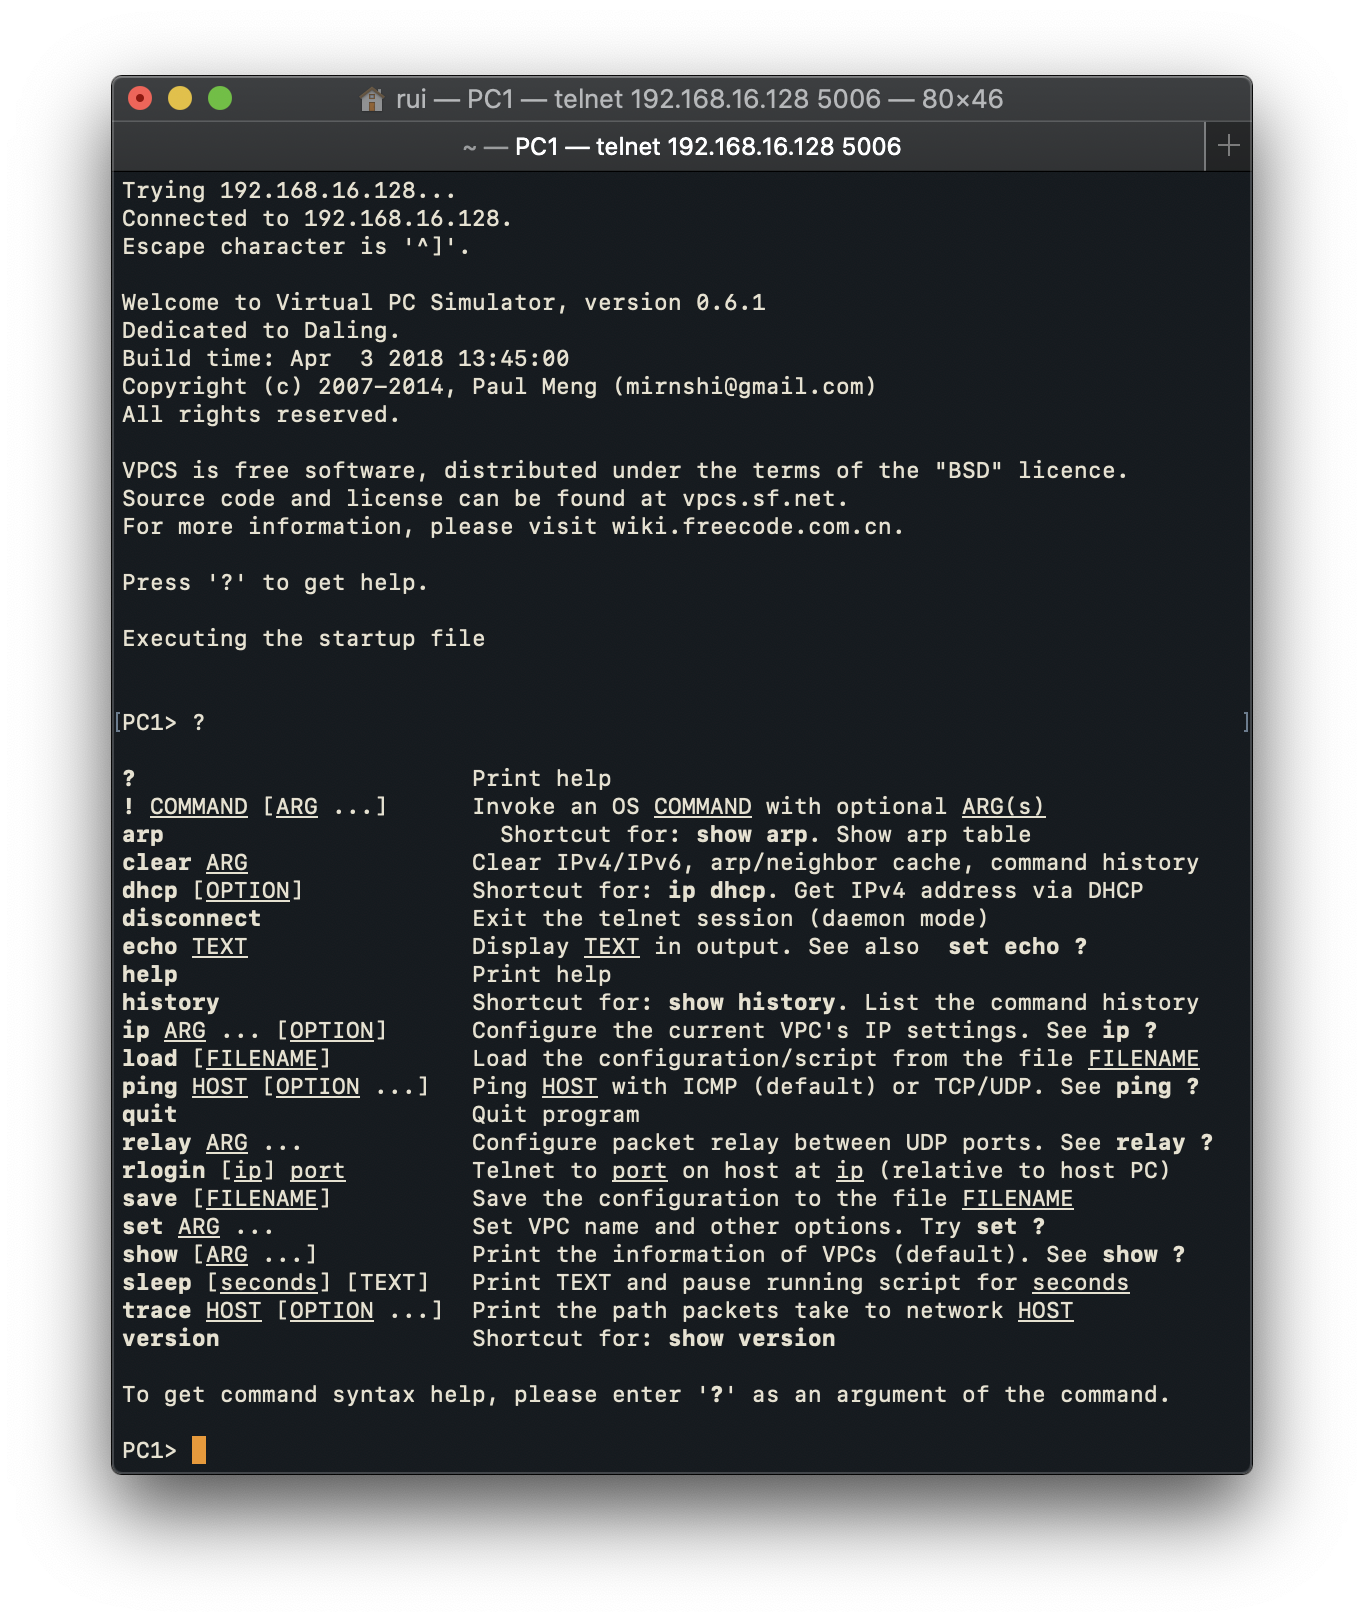
\includegraphics[width=0.6\textwidth]{gns3-vpcs-cli-help}
  \caption{A telnet session showing VPCS's list of commands}
  \label{fig:gns3-vpcs-cli-help}
\end{figure}

Due to this reason, the GNS3 project is recommending users to progressively stop using VPCS nodes and move towards Docker~\cite{ytdynamipsvpcs}.

The experiences carried out for this thesis use exclusively Docker containers as guests.

\subsection{Links}
\label{subsec:links}

A crucial part, and arguably the only element common to really \emph{any} GNS3 topology, is the emulation of data links.
For any two nodes to communicate, their \acrshortpl{nic} must be connected through a ``pipe,'' through which bits can flow in two directions.
GNS3 maintains a program, with an independent code base and which can be used independently, outside GNS3, called ubridge (in some places stylized as uBridge).\footnote{\url{https://github.com/GNS3/ubridge}}
This program is the implementation of each of the straight lines that the user can draw on the canvas, clicking on two nodes, one after the other, and selecting the interfaces on each of them, to where the link is connected, reminding of a physical cable plugged on each free Ethernet port.

A deep study of ubridge wasn't carried out to know the implementation details.
What is practically observable is that, for each link, for each running interface on both of its ends (0, 1, or 2, depending on the status of the nodes), a user-level \texttt{ubridge} process exists on the compute's OS.

These processes listen on the virtual/software interface they were plugged in and encapsulate the traffic in UDP packages and send them through the compute's host OS network stack to the \texttt{ubridge} process on the other end of the logical link (it may or may not be running on the same compute). % TODO put UDP on glossary/acronyms
Conversely, they receive UDP datagrams, de-encapsulate the traffic inside them, and ``inject'' it back on the virtual interface they are attached to.

% <IF TIME, INVESTIGATE AND BRIEFLY DESCRIBE HOW THIS ``ATTACHMENT'' WORKS> % TODO <- ver!

ubridge is known to provide functionality of configuring simulating packet loss (by frequency or percentage), time delay in packet delivery, corruption of a fraction of the packets, or a Berkeley Packet Filter (for filtering out packets matching an expression)~\cite{ubridgereadme}.

% end of section gns3emulating


% Section "Using GNS3. Practical case study"
\section{Using GNS3. Practical case study}
\label{sec:gns3practicalcasestudy}

Here, we describe the process and results of the experiments carried out to assess aspects of the feasibility, and convenience, of using GNS3 in a computer networks course comprising the use of network gear on (emulated) network configurations.

Hopefully, some of the gained insights can be extrapolated for other similar teaching facilities of slightly different characteristics.

To provide a real and well-defined set of examples to put in practice, the selected exercises and lab descriptions were taken out of the lab classes handouts for the 2018-2019 edition of ``Architecture and Protocols of Computer Networks,'' known by its Portuguese acronym APRC, an elective, graduate course offered at the Masters in Informatics at the FCT/NOVA.

\subsection{Overview of the considered labs and exercises}
\label{subsec:gns3consideredlabs}

Out of the 5 lab assignments, some of which span across more than one class, planned for a semester, only the first ones, which resort to the lab equipment to put in practice the subjects related to layer-2 and 3 switching, and ``legacy'' routing, as opposed to SDN, were considered. % TODO "span across?". Usar esta nota para pôr, se tiver ficado esquecido, referência no trabalho futuro aos exercícios de SDN que podem tirar partido de GNS3 e afins. SDN tem tem de estar nos acrónimos e glossário
Those are the exercises that, in the present, are expected to be done in the lab room, with real interconnected Cisco devices, issuing commands to the IOS command-line interface from the students' laptops.

The so-called ``lab-assignment1'' has a part to introduce the Cisco IOS and some basic commands for it.
Those are the ones to enter and escape the privileged mode, list the device's interfaces, and some other queries.
It also informs of how to load the running configuration of the device into the non-volatile memory, so that it persists after a shutdown, and how to do the opposite to discard unsaved running configurations and load the ones from the nonvolatile memory.

The second handout, ``lab-assignment2,'' is all about switching and layer-2 functionality.
It proposes a topology, expected to map the real interconnecting and physical disposition of devices in the room, of the nine switches, labels them with ``areas'' corresponding to cardinal points.
Students are then guided to answer questions about the expected behavior, e.g. in terms of reachability between hosts, according to parameters, which they should also issue in a coordinated fashion, for STP, VLANs, and trunks.

For the third lab assignment, divided into two parts, students are requested to connect their laptops to a topology similar to the one in the switching labs, but setting up the network interfaces on the nine multi-layer devices that interconnect them as layer-3 routing ports.
As written in the handout, the idea is that the routers interconnect the backbone of the offices of a nation-wide corporation.
Therefore, the computers in each bench (office), have its interface in different IP prefixes, corresponding to separate LANs. % TODO add gls reference

First, to set up set routing, students are requested to design an addressing plan, setting up prefixes and hosts on the routing interfaces connected each router to another, and then setup manually, using IOS's interface, static routes that allow to connect each office's LAN to another.
After this, students can configure the router/switch virtual interface (which is also configured to be on its respective LAN) as the default gateway and \texttt{ping} each other's computer.

The second goal is to, instead of doing the routing statically, configure the routers to use OSPF, and perform a set of analysis and variations on the exercise, such as changing the bandwidth of some links, turning other links off and foreseeing the behavior according to the specification of the protocol.

Students are also requested to use Wireshark to capture the data OSPF exchanges across the network.

\subsection{Testing environment}
\label{subsec:environment}

The testing for this component was done running the GNS3 server in virtual machines on DI's servers. % TODO acronyms?
These are machines with two Intel Xeon E5-2650~v4~@~2.20~GHz (a total of 24 cores) and 64~GiB of RAM.
The two virtual machines used to test the lab handouts' topologies are running on the VMware ESXi bare metal hypervisor, with nested virtualization enabled (needed so appliances, which are themselves VMs, can be emulated), had 4 CPU cores, and 2 and 8 GB of RAM allocated, respectively.

For the switching labs, all the nodes of the topology were set to run on the same machine.
Conversely, for the sake of testing that functionality, the routing (static and OSPF) labs were tested with the nodes distributed accross two computes (both on the aforementioned infrastructure).

% Figure fig:gns3-aprc-lab2-handout-topology
\begin{figure}
  \centering
  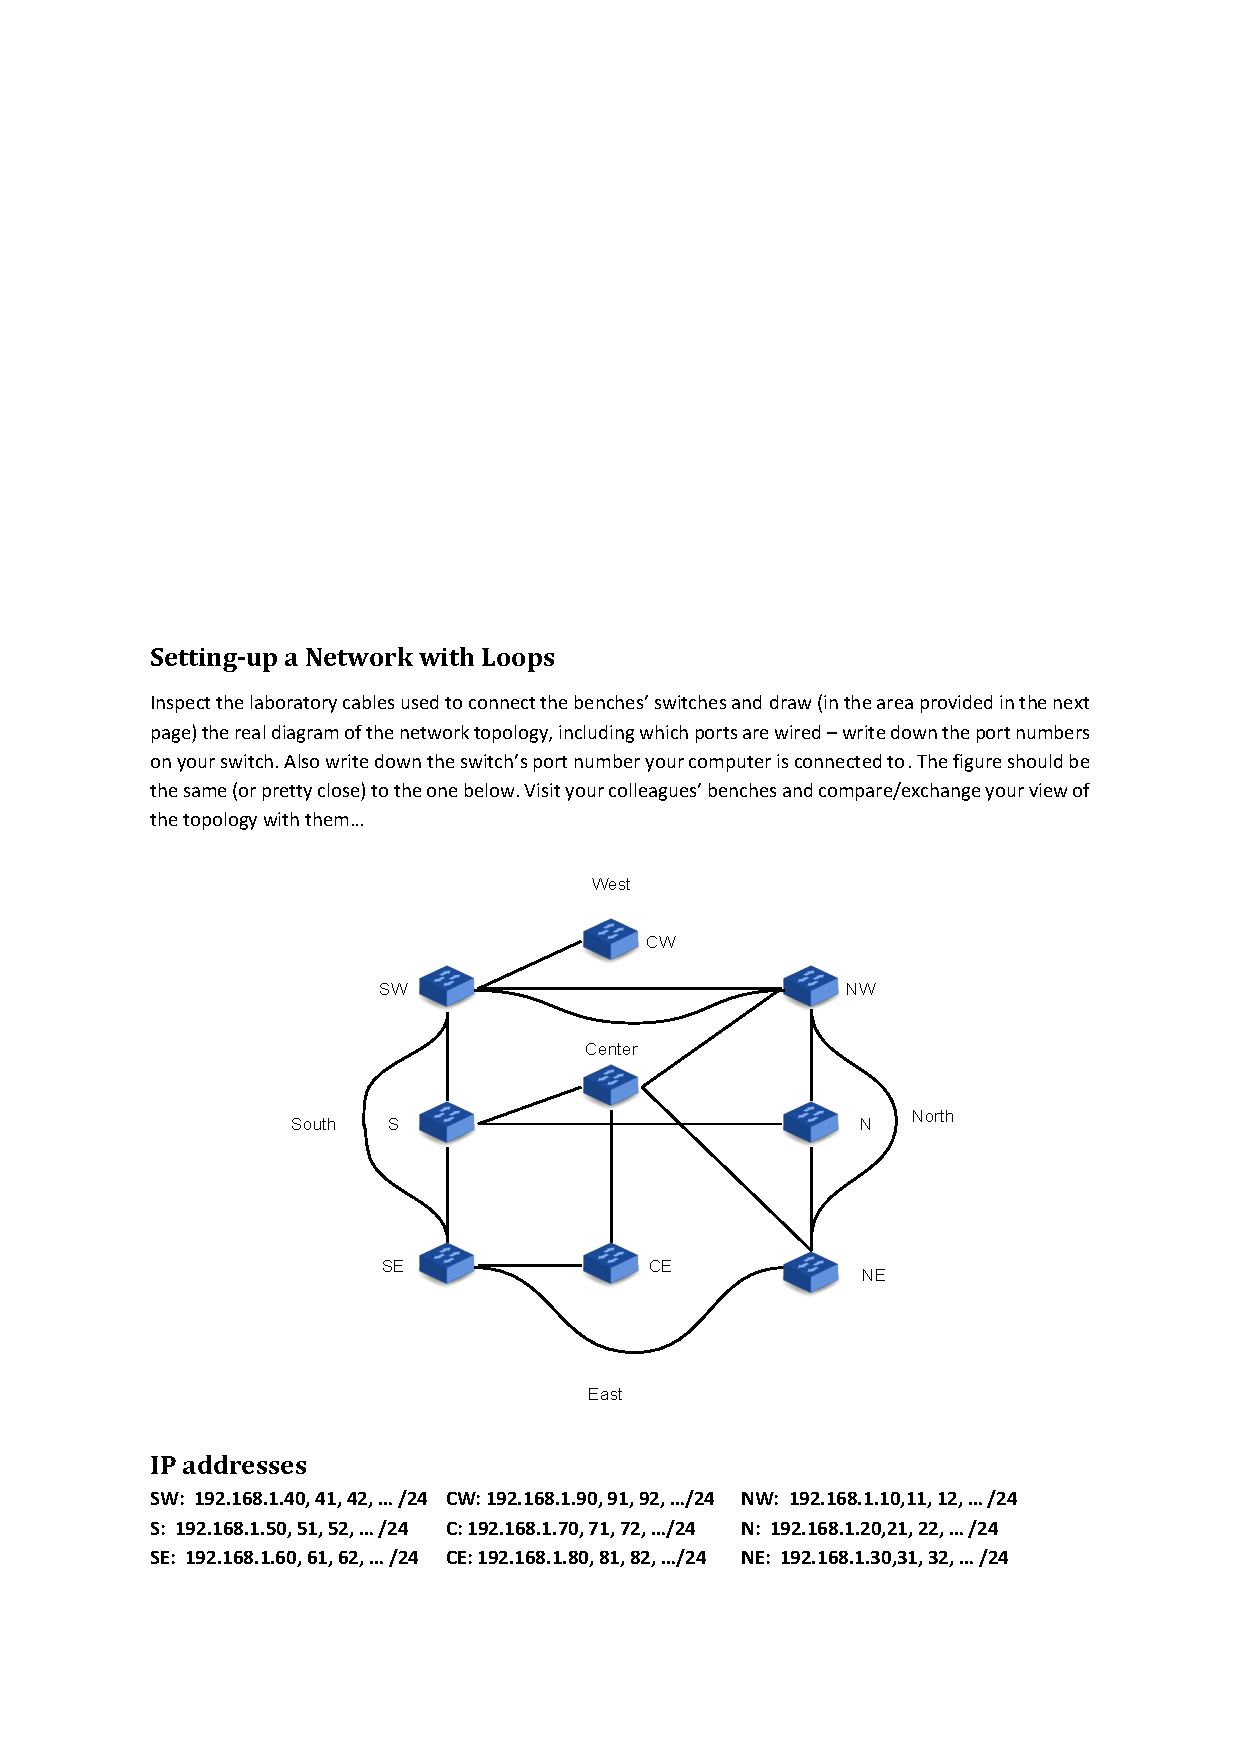
\includegraphics[width=0.8\textwidth, frame]{gns3-aprc-lab2-handout-topology}
  \caption{Section of ``lab-assignment2'' showing the topology}
  \label{fig:gns3-aprc-lab2-handout-topology}
\end{figure}


\subsection{Introduction to Cisco IOS and switching labs}
\label{subsec:gns3introswitching}

As said before, the first lab assignment introduces host-side commands (mostly Linux) and TCP/IP practical concepts such as IP address and \acrshort{mtu}, and its definition for the host's \acrfullpl{nic}.
The part of this lab handout that is to be performed on Cisco is perfectly doable on a GNS3 session with both (lighter) Dynamips EtherSwitch-enabled legacy routers or the more modern Cisco IOSvL2-3.
Double clicking on a node corresponding to one of these switches/routers, the GNS3 GUI will launch a terminal window on the user's desktop automatically executing the command necessary to create a \texttt{telnet} session to the node.

To perform the second lab, the topology described in figure~\ref{fig:gns3-aprc-lab2-handout-topology} (a section of the handout document) is physically implemented in the lab room with Cisco Catalyst switches interconnected accordingly with UTP-Ethernet cables supporting the data links.
The topology has loops which STP, running in the switches, is expected to eliminate by disabling certain link(s).
Part of the exercise is to foresee, according to the protocol's specification, which one(s) will be shutdown.

Execute this exercise in GNS3 already poses a bit of challenge, and introduces a dilemma.

Using the recommended IOSvL2 appliances on a typical laptop is not \emph{easy}.
First of all, IOSvL2, which as told before, runs on QEMU/KVM, is only supported on GNU/Linux computes.
On a laptop setup with macOS or Windows the standard GNS3 installation recommends having VMware Fusion or Workstation, respectively, installed and downloading the so-called GNS3 VM, which nothing else than a VM image, optimized for VMware's desktop hypervisors, containing a pre-made installation of the GNS3 server on an Ubuntu Server LTS.
The GNS3 GUI for macOS and Windows then facilitates setting up the ``GNS3 VM'' to not need to setup a generic remote server to be used as compute, and is also able to open VMware Fusion or Workstation in the background and power on the GNS3 VM, as a means to offer a standardized compute node.
Needless to say, this does not come without its overhead, both in terms of performance and practicality.

On the other hand, using a Dynamips EtherSwitch, that can be run on Dynamips directly on a macOS or Windows installation, and is much, much lighter, is not recommended anymore, since it requires legacy Cisco images, may not provide all the functionality, is reported to have bugs, etc.

In practice, though, if students have access to the IOS images compatible with the school's labs switches, all the exercises were proven to be performable on a laptop using Dynamips nodes.
VLANs are supported by these images, as well as STP, and standard routing protocols, such as OSPF (covered on a lab assignment too) are also run without problems on these equipments.

Summarizing, using Dynamips is no longer encouraged.
However, one assumes that the advice seen on the GNS3 forums, and on the videos and interviews with Jeremmy Grossmann already cited, for not using Dynamips is very much centered on advanced features and IOS interface compatibility.
However, in an undergraduate or graduate university level, where applying theoretical principles and seeing and doing in practice, in a controlled environment, not bound to any vendor tools, this advice may very well be irrelevant.

That said, Dynamips ensures actually better throughput on its EtherSwitch modules (surpassing the FastEthernet 100Mbps barrier) with a simple \texttt{iperf3} test between two hosts connected to the same device than an analogous scenario with IOSvL2 switches. % TODO add screenshot or something?
It also is dramatically lighter on resource consumption, and users can emulate such nodes on their macOS or Windows---and obviously on GNU/Linux, which supports GNS3's emulation alternatives fully, too---without having any need for a distributed or load balanced architecture.

\subsection{Routing and OSPF on Cisco routers}
\label{subsec:gns3ospfrouting}

Although the considerations related to using Dynamips versus using IOSv are also applicable here, the complexity of this exercise will be used to demonstrate two facets of GNS3's functionality and setup-wise flexibility, namely:
\begin{itemize}
  \item Distributing the load between many servers (computes)---useful to scale, and particularly necessary when emulating heavier nodes such as IOSv instances.
  \item Topology snapshots
\end{itemize}

For a large topology, since GNS3's emulation is quite heavy (more details on that later), distributing the load may be necessary to make an emulation feasible.
GNS3's topologies are JSON files describing which devices exist on it, their names, meta-information to be used in the moment where each emulator is executed, and which links connect which virtual interfaces~\cite{thebookofgns3}.
Therefore, there is not a practical limitation for the central points, the controller and the GUI, in the size which a topology can have.
It is possible, and examples across the web are given, of enormous topologies.

The real burden is on the computes, which symbolize each host where virtual routers and guests run.
To balance the load, one uses separate hosts to run an instance of the GNS3-server, in the role of a compute, receiving instructions from the controller (in turn controlled by the user using, for instance, the GNS3 GUI) to interact with the running emulators.
As long as the total amount of emulators and ubridge processes attached to those processes running on each of those hosts doesn't use too many resources of each compute-host, there isn't exactly any bottle-neck, since the emulated nodes execute independently of GNS3's ``brains''.

Unless the user is editing the topology, creating or deleting nodes and links, starting and stopping machines, or other orchestration-specific tasks, the interaction with the running nodes is done thought direct \texttt{telnet} connections to the emulator processes from terminal windows accessible to the user, outside of GNS3.
To make that easier, if using the GNS3 GUI, a user can double click on e.g. a ``powered-on'' switched or Ubuntu Docker Guest, and a helper is transparently executed which will open a terminal window on that (graphical) host, automatically running a command like \texttt{telnet 10.170.138.106 5001}---where \texttt{10.170.138.106} is the IP address of the compute host where a certain node is running and \texttt{5001} is the concrete TCP port where the emulator process is listening to accept connections to the console.

In the case of the lab assignment 3 (layer-3 routing and OSPF), the (virtual) servers were set up in the way illustrated by figure~\ref{fig:gns3-ospf-lb}.
One was running the GNS3 server as the controller (and also as compute for some nodes), and the other only as a ``secondary'' compute node.
Note that there is no reason to assume that the ``primary'' (generally, the controller) is the host with the most resources.
In fact, this wasn't the case in the architecture set up for this experiment.

% Figure fig:gns3-ospf-lb
\begin{figure}
  \centering
  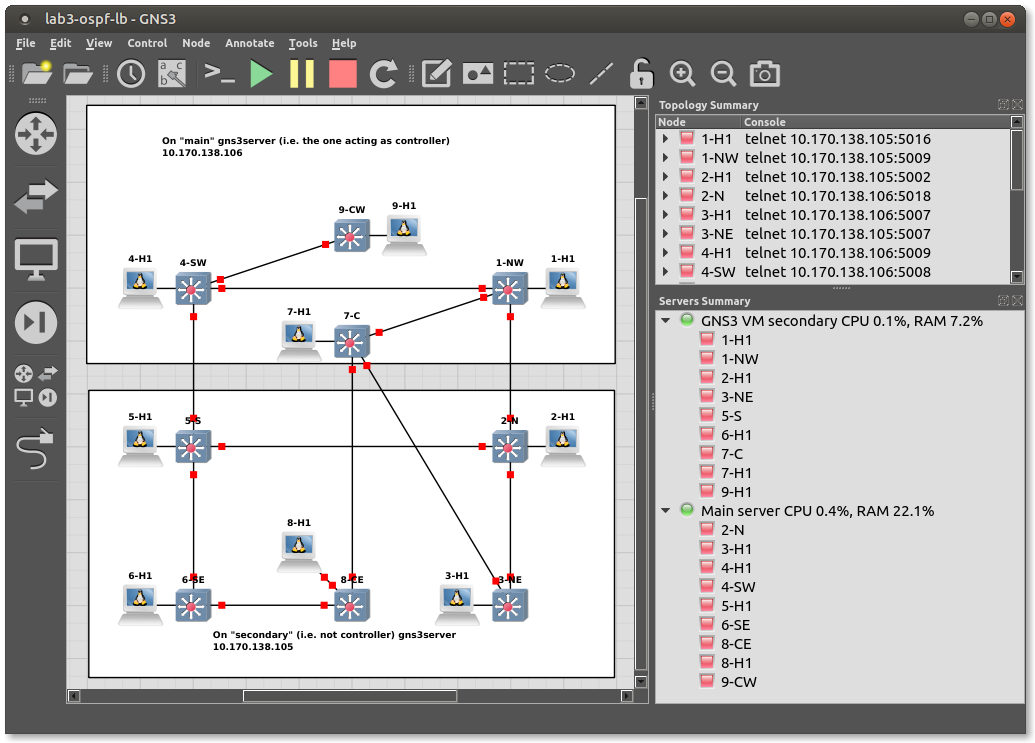
\includegraphics[width=0.9\textwidth]{gns3-ospf-lb}
  \caption{View of load-balanced lab~3's topology in GNS3 GUI}
  \label{fig:gns3-ospf-lb}
\end{figure}


% end of section gns3practicalcasestudy


% end of chapter

  % % !TEX root = ../Thesis.tex
% !TEX spellcheck = en-US

\chapter{Kathará}
\label{ch:kathara}

In this chapter, Kathará is explored. It is the other example of a network emulator to be studied in depth, to analyze its implementation and assess its suitability in functional and non-functional aspects for usage as replacement for the University's physical laboratory.

As said before, Kathará is a new implementation of Netkit, done from the ground up, which shares the same declarative language for preconfiguring labs (both the topology in terms of nodes and ``links'', as well as the default behavior and configuration of each node) with the latter, using an almost identical command-line interface.

% Despite having being developed to deploy very different kinds of networks than those of Netkit, namely software-defined networks, those with programmable data plane nodes, and with virtual network functions, Kathará is recommended as a successor by its precursor's website, since it promises total backwards compatibility, while having a more portable and efficient architecture, thanks to relying on Docker.

The structure of this chapter is as follows: in the first section, Kathara's functional capabilities are described from a high-level vantage point, as well as its user interface; then follows a lower-level explanation of this emulation framework's architecture and implementation; finally, a case study identical to the one applied to GNS3 on section~\ref{sec:gns3practicalcasestudy} is presented.

% Section "UI and functionality"
\section{UI and Functionality}
\label{sec:katharafunctionality}

% To build such a framework, the chosen starting point was an experimental tool called sdnetkit, which enhanced Netkit with OpenFlow enabled switches, still explicitly supporting ``traditional routers'' performing distributed routing protocols like OSPF~\cite{sdnkit}.
% Kathará then evolved to be a fully backwards compatible tool with Netkit, using the same conceptual philosophy in terms of interfaces and emulated topology definition, with a substantially different implementation, and the capabilities mentioned earlier in this section.

The high-level functional capabilities of Kathará explored in this work are the exactly the ones shared with the original Netkit---i.e. building and emulating topologies with traditional routers and switches and generic hosts.
However, as will be seen later, the implementation changes and overall modernization that Kathará brings can benefit any user.

As a side-note, it's important to point out that Kathará officially provides a very comprehensive repository of hands-on labs,\footnote{\mbox{\url{https://github.com/KatharaFramework/Kathara-Labs}}} mostly in the form of a PDF containing a sequence of slides and an archive with a shareable Kathará lab with part of the work done, so that many didactic topics in networking, from traditional routing to \gls{sdn}, NFVs, and ``behavioral model'' (P4 language), can be followed step-by-step, with some theory in the middle.
The first one of those ``labs'' is the `Introduction to Kathará,' referred to afterwards.

% Figure fig:kathara-topologynodes
\begin{figure}
  \centering
  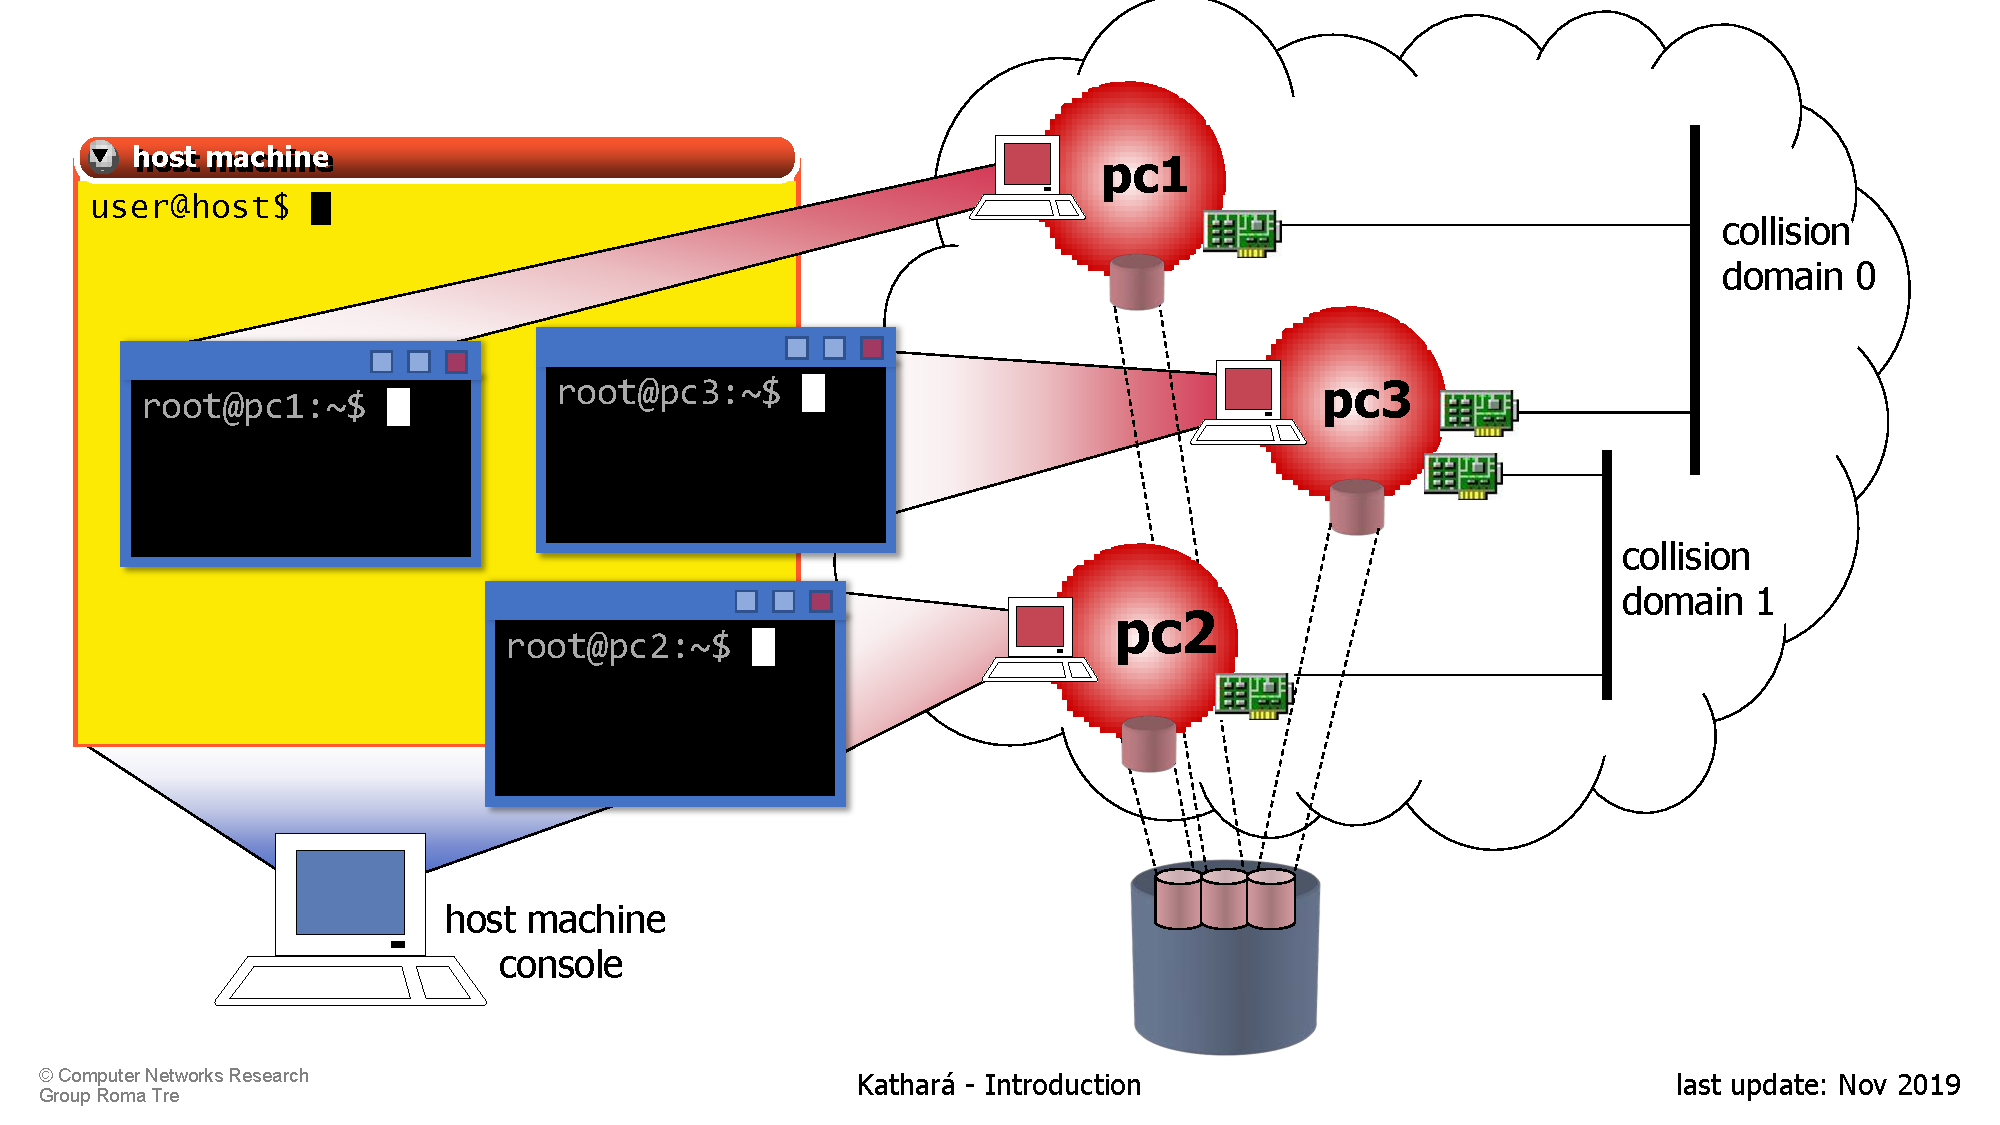
\includegraphics[width=0.8\textwidth,frame]{kathara-topologynodes}
  \caption{Slide taken from `Introduction to Kathará' showing a simplified lab in action}
  \label{fig:kathara-topologynodes}
\end{figure}


As stated in `Introduction to Kathará,' each (emulated) device has:
\begin{itemize}
  \item a console (a terminal window) which gives access to a \texttt{bash} shell inside the container
  \item an (virtually) isolated memory
  \item an (virtually) isolated filesystem, though Kathará provides a way to mount shared files among the nodes of the lab, via a convention of directory hierarchies so no explicit configuration is needed
  \item zero, one, or more network interfaces
\end{itemize}

The slides also explain that each network interface can be connected to a (virtual) collision domain and each virtual collision domain can be connected to several interfaces.
All this is illustrated by figure~\ref{fig:kathara-topologynodes}.

Kathará's interface has two parts: a set of commands that can be issued in the host (the machine where the emulator is being executed) shell, and the a structured way to define labs, which includes a syntax for defining topologies---i.e. which nodes are there, what are their names, how many network interfaces do they have and to which collision domain (i.e. links) are they connected to---and also a conventionalized way to structure configuration files that are automatically read by the software inside the nodes, like IP configurations or routing parameters.

These interfaces are not exhaustively exposed in this work since that would just mean duplicating the documentation resources, which are easily accessible and very clear.
However, figure~\ref{fig:kathara-topologynodes} serves as a way to illustrate, in contrast with graphical interactive tools, the way topologies are described and allows to take an immediate conclusion: to have only point-to-point links, this means that only each two interfaces that are connected via that each link need a separate collision domain and local-area networks of interconnected $N$ Ethernet-equiped hosts need a switch between them.

What was just said poses a question that will be further explored in the practical case study (section~\ref{sec:katharapracticalcasestudy}): there aren't conventional (layer-2) switching labs in the aforementioned repository, and the routing ones assume that more than one hosts sharing the same IP-prefix simply share collision domains.

% Figure fig:kathara-topologynodes
\begin{figure}
  \centering
  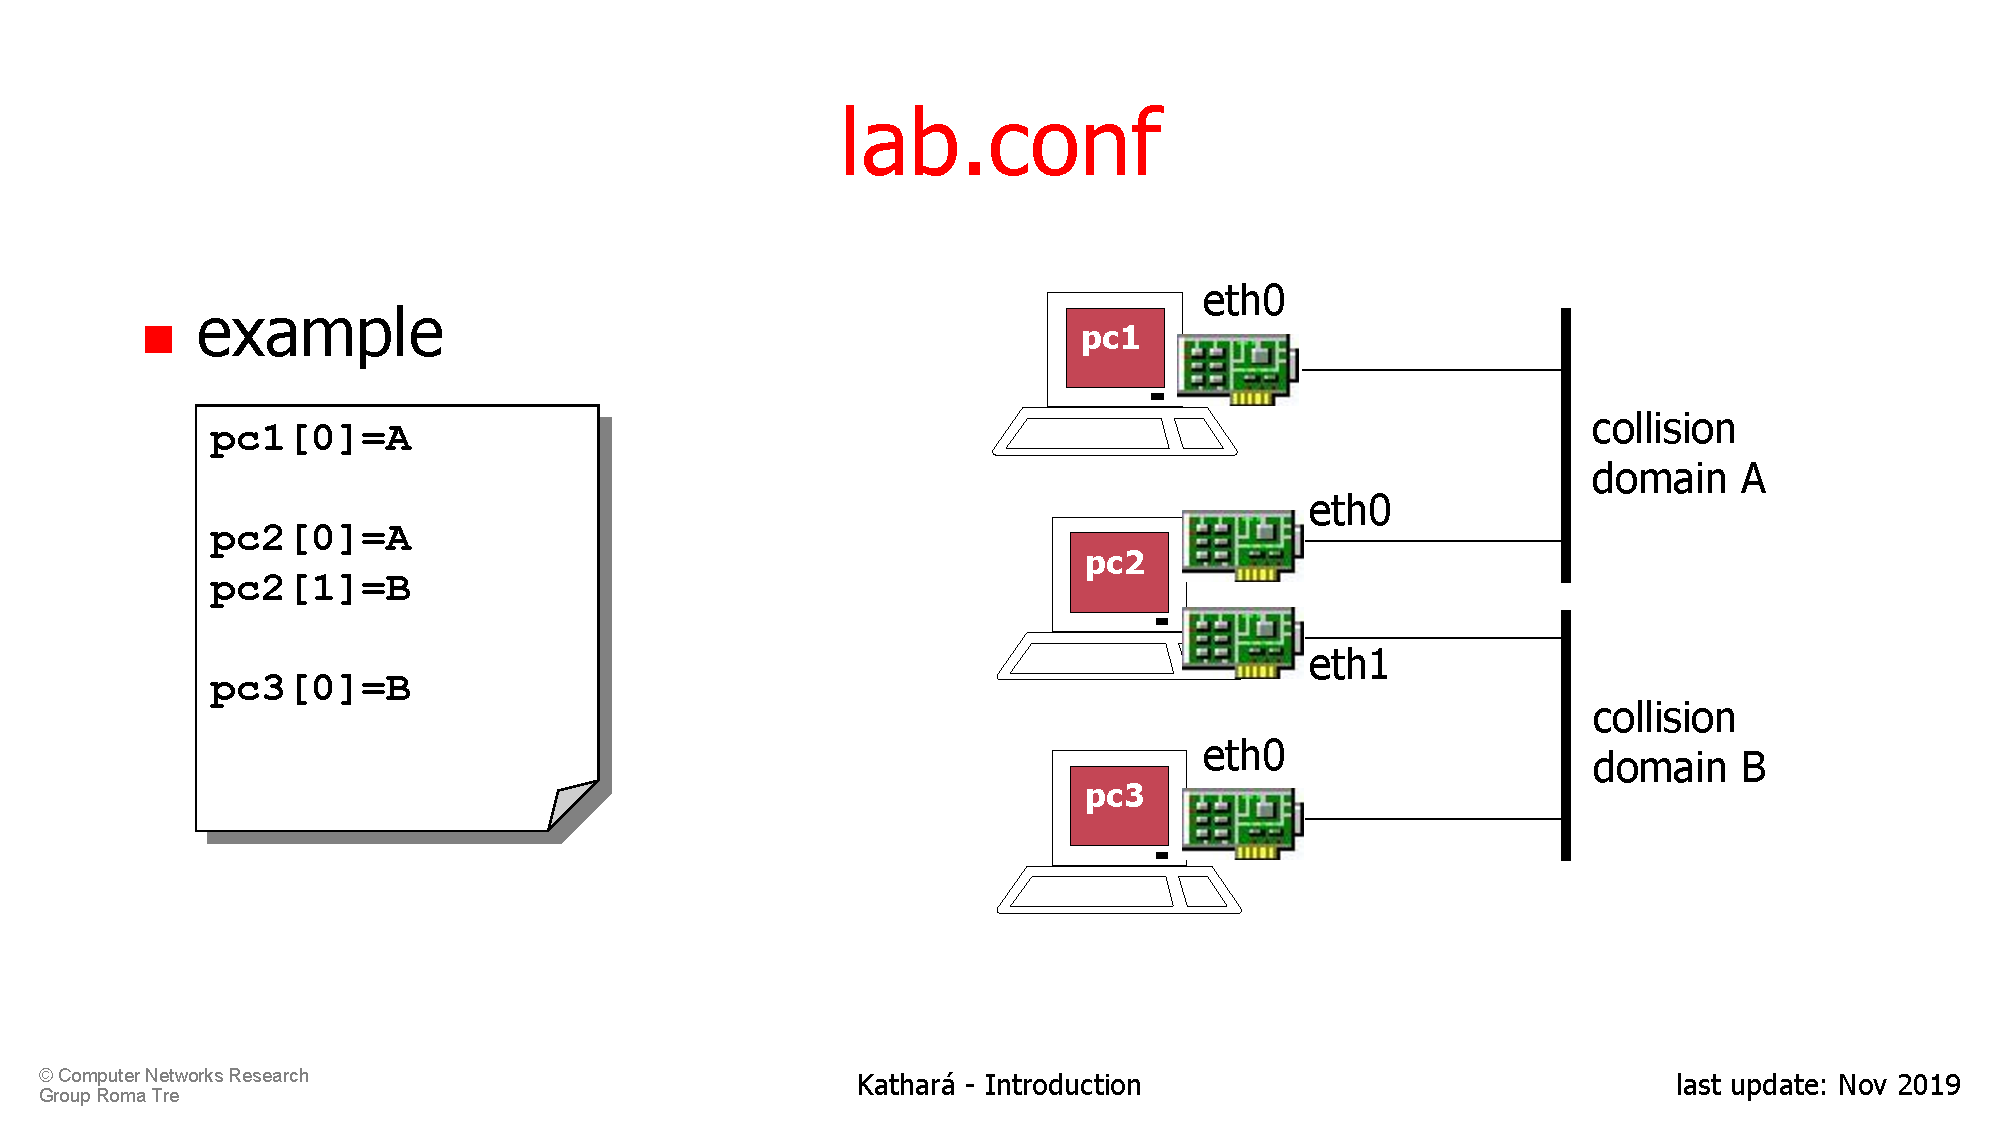
\includegraphics[width=0.8\textwidth,frame]{kathara-labconf}
  \caption{Slide taken from `Introduction to Kathará' showing the mapping between \texttt{lab.conf} and the instantiated topology}
  \label{fig:kathara-labconf}
\end{figure}


% end of section katharafunctionality


% Section "Technical overview"
\section{Technical Overview}
\label{sec:katharatechnicaloverview}

In Kathará's original announcement's paper~\cite{kathara}, the described technical infrastructure of the program, which can easily be confirmed by consulting the available Python source code,\footnote{\mbox{\url{https://github.com/KatharaFramework/Kathara}}} clearly states the basic design decision that follows the choosing of lightweight containers via Docker: every node in the topology is a Docker container.
Kathará, therefore, works as an orchestrator of containers, the same way that Docker's own Compose\footnote{\textquote{Compose is a tool for defining and running multi-container Docker applications \ldots\ with a single command, you create and start all the services from your configuration.}~\mbox{\url{https://docs.docker.com/compose/}}} is.
The difference is that, while Docker Compose exposes a limited set of network parameterization, given that its purpose is to handle the combination of different application-level services running in containers that must be able to exchange IP traffic between each other, Kathará uses lower-level primitives exposed by Docker itself to setup the containers' virtual interfaces and hook them up to virtual collision domains which serve as a shared medium between any number of nodes, and therefore constitute links or hubs in a topology.

% Figure fig:kathara-architecture-paper
\begin{figure}
  \centering
  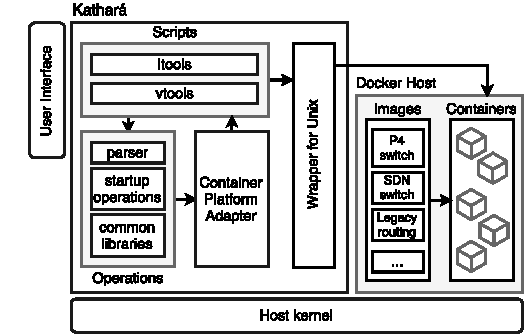
\includegraphics[width=0.8\textwidth]{kathara-architecture-paper}
  \caption{The diagram where Kathara's authors present its architecture}
  \label{fig:kathara-architecture-paper}
\end{figure}


Kathará's own architecture, depicted in figure~\ref{fig:kathara-architecture-paper}, is decribed as comprising three parts:
% Scripts, Operations, and Container Platform Adapter
\begin{description}
  \item[Scripts] used by the users to interact with Kathará.
  These scripts implement the basic operations that are used to start, stop, and pause the network nodes defined in the Kathará configuration and are divided into the two categories referred to in section~\ref{sec:katharafunctionality}, the \texttt{ltools} and the \texttt{vtools}.
  \item[Operations] is a module which \textquote{includes a set of utility functions that are used by the Scripts module in order to allow Kathará to interpret the configuration provided by the users.}
  This module is made of three main logical components: \emph{parser}, \emph{start-up operations}, and \emph{common libraries}.
  The parser is responsible by translating the textual configuration into a network topology; the start-up operations component ensures the cross-system compatibility, namely copying the files that must be copied to inside the nodes;
  \item[Container Platform Adapter] is a layer between the Operations module and Docker, which could allow to use different container platforms other than Docker.
\end{description}

To separate different kinds of nodes with different specific needs in terms of the software (e.g. daemons available to be run) running on them, Kathará allows for its topologies to specify which Docker image it should be running.
The default one (which can be changed on the program's preferences) is \texttt{kathara/quagga}. Therefore, all nodes, are able to launch any of Quagga's functionality, even if they, by omission, don't do it.
For P4 or \gls{sdn} enabled switches, two different images exist, as well as for the ClickOS-enabled one for creating \glspl{vnf}.

The Docker networking mechanism~\cite{dockernetworking} to create the collision domains through which interfaces of different containers communicate with each other is not explicitly stated in Kathara's paper.
Therefore, to be sure, one would need to look into the corresponding module on Kathara's source code.

% Kathará also leverages the notion of Docker images, available via Docker Hub or just setup locally on the user's Docker installation, both for separating the functionality (and ``role'') that different kinds of nodes may have on a lab (from being a traditional router to an OpenFlow switch, or an end-host running a RDBMS). % TODO first, take this out of here (maybe to the practical case study, when mentioning the way to create an inherited image), then add RDBMS to the acronyms

% end of section katharatechnicaloverview


% Section "Using Kathará. Practical case study"
\section{Using Kathará. Practical Case Study}
\label{sec:katharapracticalcasestudy}

For the practical case study of Kathará, we followed the same approach than for GNS3's, used the same laboratory handouts from APRC as reference, but implemented in Kathará's different paradigm.
Refer to section~\ref{sec:gns3practicalcasestudy} for an overview of the labs and their topics.

\subsection{Setting Topologies in Kathará}

As mentioned earlier in this chapter, Kathará doesn't offer a graphical interface to draw topologies, and nodes added and removed, started and stopped, and text-based consoles to them are created via a set shell commands.

We mentioned as well that, in Kathará, there aren't end-to-end links as such, like there are on GNS3.
Instead, Kathará has collision domains, which are Ethernet media, shared by whichever interfaces are attached to them, and all hosts connected through a collision domain can have packets sent back and forth among each other.
For instance, each IP-prefix corresponding to a logical LAN, connected to a layer-3 router, can have all its hosts attached to the same collision domain.

In spite of the aforementioned, to be coherent with what was done in the GNS3 case-study and to be able to compare both frameworks more fairly---and because it is a condition to perform the switching assignment, in lab handout~2---it was decided that we would always use point-to-point links, which in practice means creating as many collision domains as there are links, and attaching each corresponding pair of interfaces in the nodes to every correct one. % TODO este point-to-point está certo?

% Figure fig:kathara-annotated-lab3-topology
\begin{figure}
  \centering
  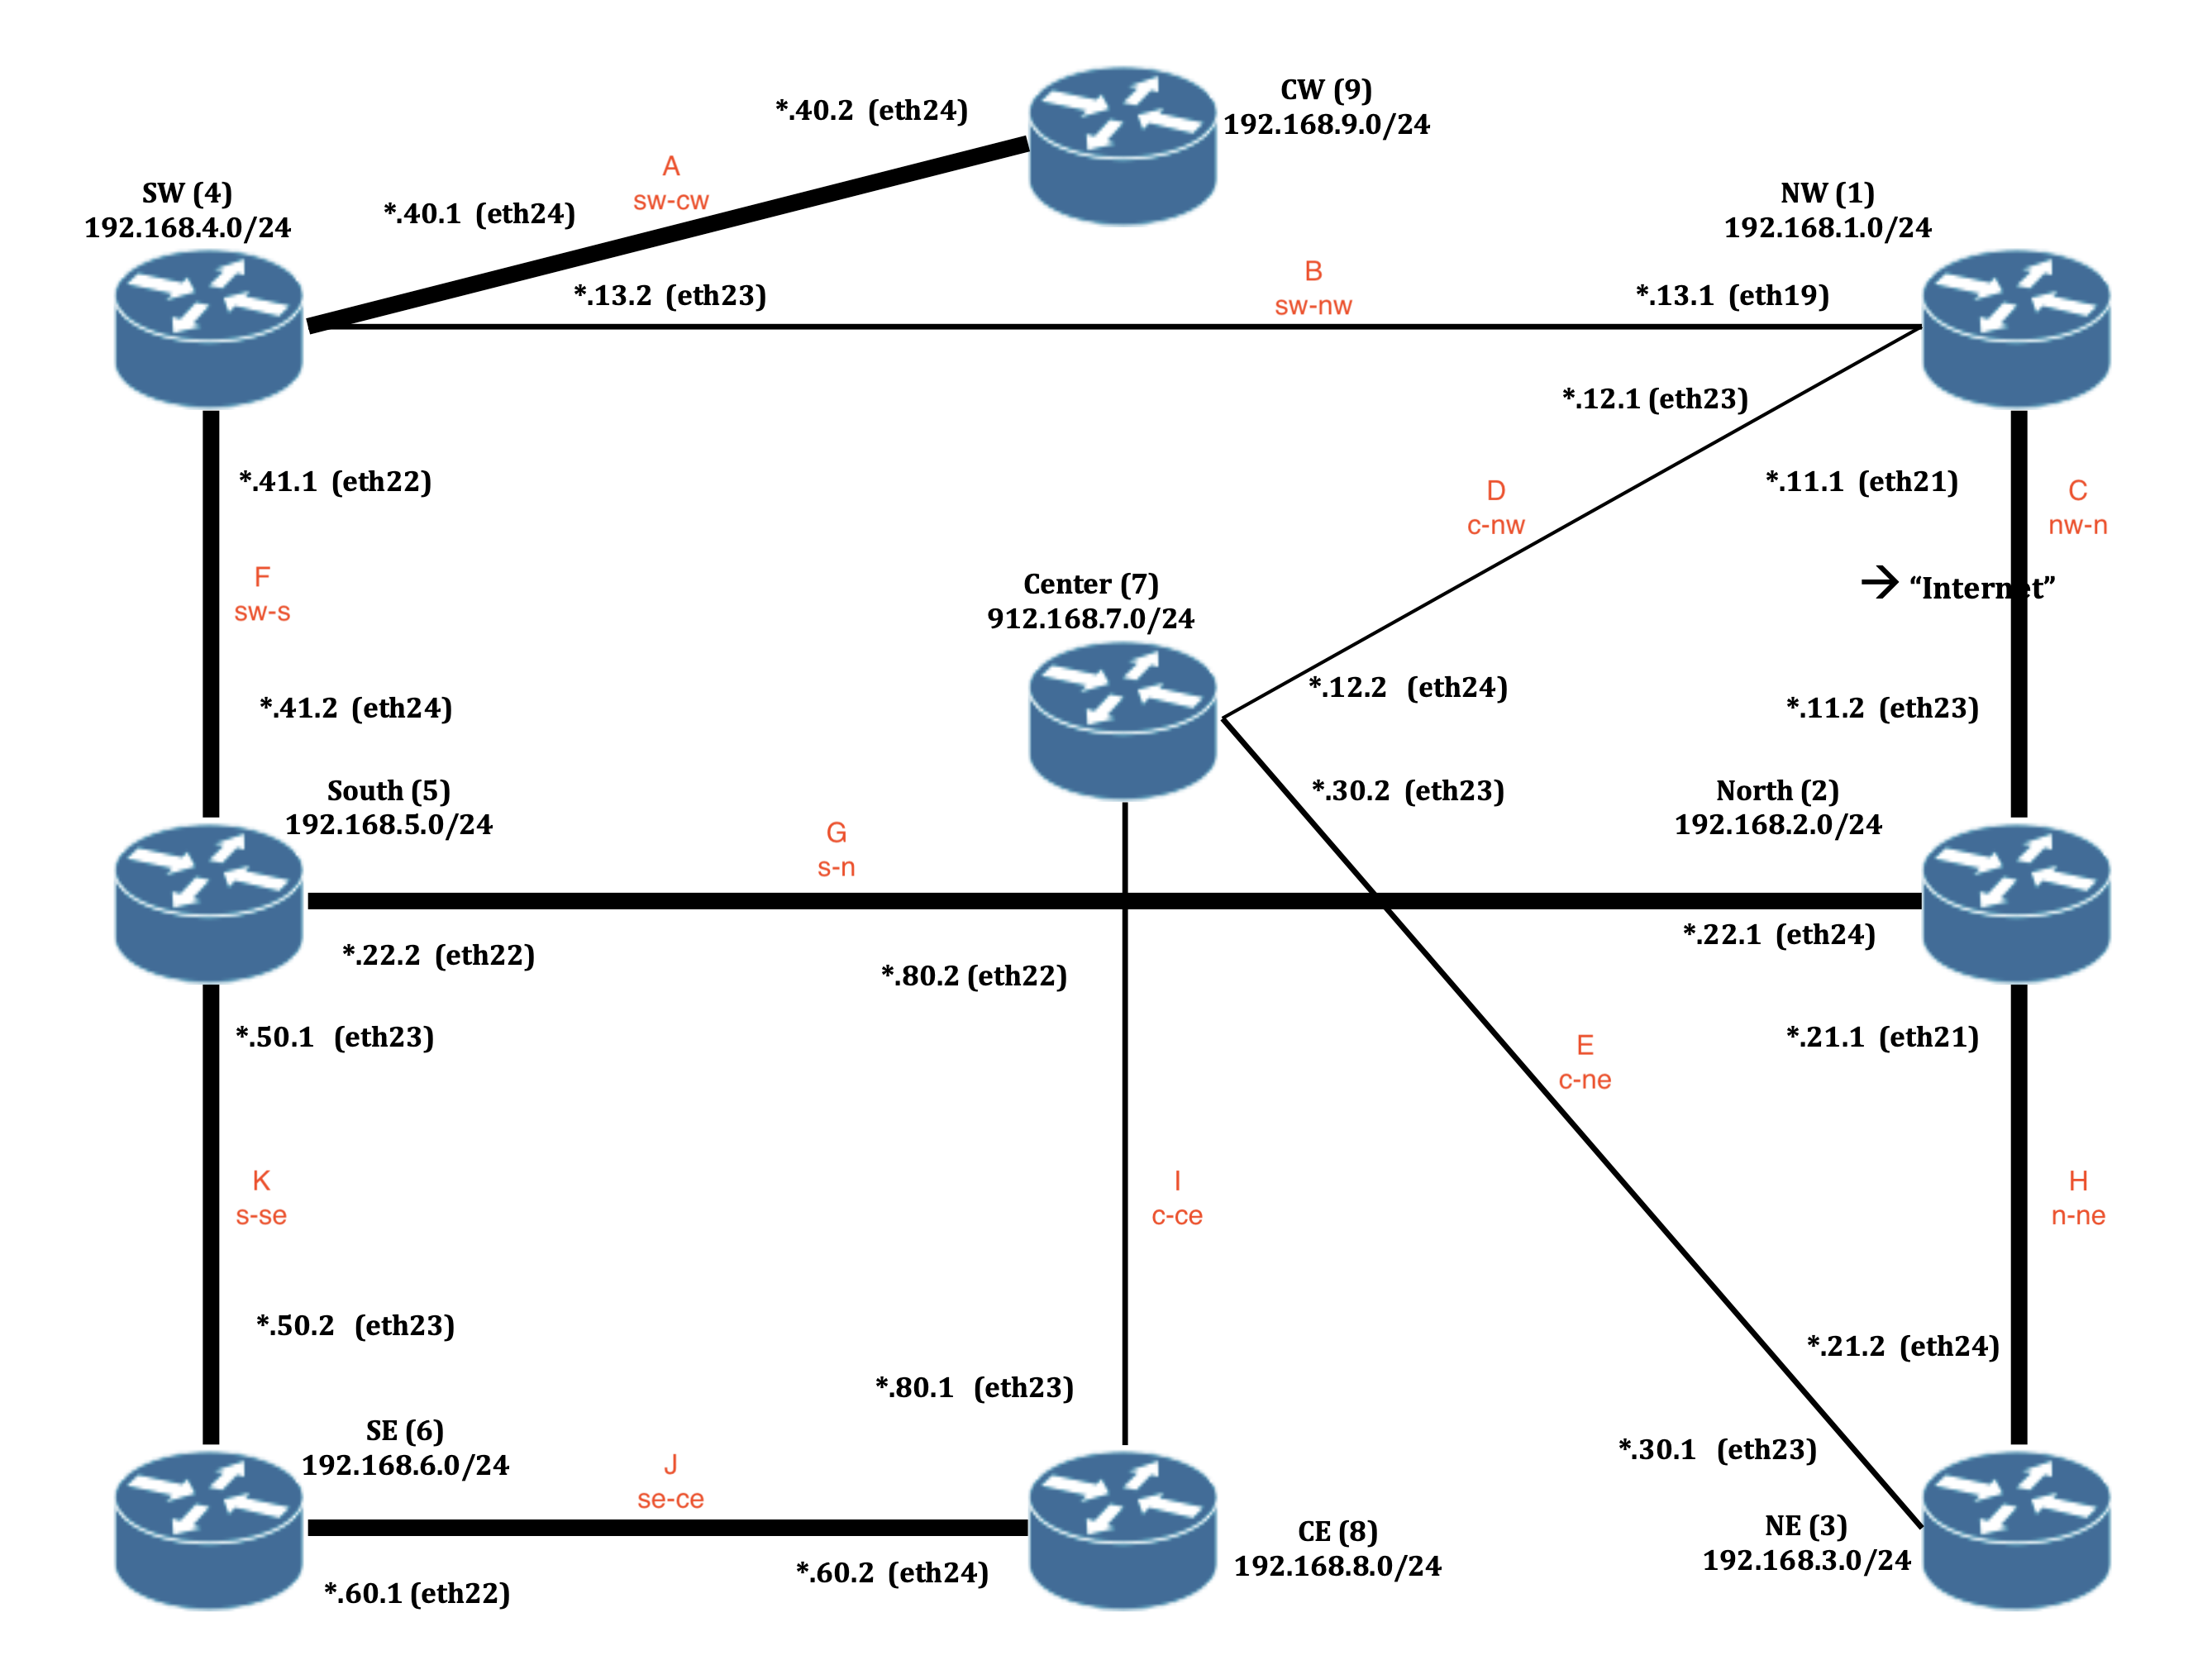
\includegraphics[width=\textwidth]{kathara-annotated-lab3-topology}
  \caption{Section of ``lab-assignment3'' showing the topology, with every collision domain annotated}
  \label{fig:kathara-annotated-lab3-topology}
\end{figure}


To facilitate this process, the graphical representation of the topology as given in the course's handout PDF was annotated with the letters that are becoming each collision domain, as figure~\ref{fig:kathara-annotated-lab3-topology} depicts. % TODO fazer versão vectorial desta figura
Then, writing Kathará's \texttt{lab.conf} and making sure that it is correct becomes much easier.

\subsection{Switching Exercises}

The switching lab was set up using a similar methodology than the one described just before for lab~3---i.e. the topology was graphically annotated to define the collision domains among the several interfaces.

Then, using Kathará's convention to ``pass-on'' configuration directories to each container, we defined the startup file (that is executed by its respective container when it ``boots up'') to setup a bridge virtual interface, according to the Linux bridge documentation and online resources~\cite{brctlman,howtobridgelinux}.

The configurations, both the \texttt{lab.conf}, which defines the topology, and one of the nine (the other ones are analogous and only vary in the number of interfaces) \texttt{<node\_name>.startup}, are shown as examples in the listings appendix as listings~\ref{listlab2conf} and~\ref{listlab2startup}, respectively.

For the switching exercises, we found out that there is some kind of limitation, either in Docker itself, in Docker's chosen intercontainer networking strategy, or in Kathará's implementation.
The containers (lightweight virtual Linux hosts), equipped with multiple \glspl{nic} that perform each switch, are not capable of successfully performing the Spanning Tree Protocol, which is demanding for a topology with a loop, which the exercise deliberately has.
We were not able to find a convincing explanation for this fact.

\subsection{Working Under Load and Version Control}

Kathará doesn't provide any \textbf{load balancing} mechanism out of the box.
Containers are expected to run under one single Docker host.
On the one hand, one can try to imagine ways to tunnel the traffic from certain nodes to any arbitrary different topology, by bridging virtual Docker interfaces to some of the hosts' interface.
On the other hand, as exposed in more detail later on, Kathará doesn't demand nearly as many resources for a large topology as GNS3.

Regarding \textbf{version control} (what, in GNS3, is achieved via \textbf{snapshots}), Kathará's approach is different.
Every relevant configuration is expected to be written, either in the configurations passed in conventionalized sub-directories of the project to the hosts to configure the routing daemons or any other software running in the container, or in the declaration of the graph in the \texttt{lab.conf}.
All of these are plain-text files, therefore the user is encouraged to resort to a version-controls solution, like Git\footnote{\url{https://git-scm.com}}.

\subsection{Performance measurements}

For completeness, we measured the host to host bandwidth in Kathará, measured with \texttt{iperf3}, like shown, in the case of GNS3, in~\ref{tab:gns3-iperf}.
The values are consistently~$\approx 25.0~\mbox{Gbit/s}$, even on 1~Gbps virtual \glspl{nic}.

A measure of the OSPF convergence time for this emulator was not performed.

% end of section katharapracticalcasestudy


% end of chapter

  % % !TEX root = ../Thesis.tex
% !TEX spellcheck = en-US

\chapter{Comparative analysis}
\label{ch:comparative}

In this chapter, the results of the in-depth study of and experimentation with GNS3 and Kathará (chapters \ref{ch:gns3} and \ref{ch:kathara}, respectively) are exposed in a comparative way, so that the strength and weaknesses, some in general, or in an absolute point of view, but especially for the application intended in this thesis, which is teaching, learning, and studying in the context of university courses.

% Section "Functionality"
\section{Functionality}
\label{sec:comparativefunctionality}

Functionality, in particular in the emulated network-nodes,\footnote{By contrast with end-nodes, which no matter the technology are expected to be, in some sense, generic virtual, isolated hosts running a typical end-host operating system, and therefore are of least concern in this sense} is defined, in this document, in two senses:
\begin{enumerate}
  \item From a \emph{higher-level} perspective, the possibility to run \emph{generically} existing algorithms and protocols, exchanging packets in the respective layers according to the standard way to do so.
  \item From a \emph{lower-level} point of view, the ability to run vendor-specific software, with all of its particular attributes, maybe proprietary optimizations, augmented headers, or any kind of functionality that a particular ``brand'' of networking software may offer.
\end{enumerate}

\subsection{Higher-level functionality}

In terms of the \emph{higher-level functionality}, most general-purpose emulators, which GNS3 and Kathará are at heart, don't differ much.
Both have a way to define arbitrary topologies and store them in the filesystem and the topologies describe nodes, default configuration of the nodes, and hosts represent ``computers'' that, according to the specifics of the software/firmware they are running and number of interfaces serve as switches, routers, end-hosts running application software (client/server, P2P, etc.), or even other kinds of nodes seen in real-world networks, often called middleboxes, not studied in the present work.

An important limitation with Kathará has to be noted, though.
Among all the documented labs, none is related to bridging/layer-2 switching.
With Netkit, Kathará's precursor, whose implementation technologies were different, that wasn't the case---and exercises to test the working of STP in a switched network were documented.
In fact, if we try to mimic those labs, as well as APRC's lab2-handout (cf.~\ref{sec:katharapracticalcasestudy}), they don't work---despite capturing network traffic between nodes shows that STP is communicating, the Linux bridges.

Thus, as far as our experiments go, for layer-3 switching (data-plane) and routing (control-plane), every APRC exercise can be done with a mix of virtual Cisco gear and Linux guests in GNS3 \emph{can} be done with a Kathará lab.
And, judging by the documented labs offered by Kathará itself, many more intra- and inter-domain routing protocols, quality of service, and other things can be performed without an issue.
However, the same cannot be said for experimenting with switching network. % TODO acho que se pode dizer que isto em princípio pode ser debugged e corrigido, no trabalho further work, ou propor que isos se faça

\subsection{Lower-level functionality}

If, for example, running Cisco software is a requirement (as is the case for the company's official certifications), Kathará itself cannot accommodate it.
On the contrary, there aren't officially supported GNS3 appliances, running on any kind of platform, to run Quagga out of the box.
This is to show that, \textbf{in an academic context}, where protocols and algorithms are the subject of the study, and not vendor-specific details, \textbf{Kathará has the advantage of doing without pricey licenses and vendor lock-in}.

The degree of flexibility of the two emulators is different, due to reasons probably obvious by now.
On the one hand, GNS3 is ``a suite of \emph{emulation methods}'' (and even more than that, giving the diversity of software packages that are inside a normal installation of the software on a desktop), and offers the ability to emulate nodes using large span of technologies that don't typically work with each other by making ensuring that one single software package, uBridge, is pluggable to each of them, being responsible to handling the transmission of the traffic, in a way that each node's emulation method is never aware of the emulation method on the other end of a virtual link.
On the other hand, Kathará doesn't use any application-level data-link emulation, and requires that every kind of software, be it for switching/routing nodes, middleboxes, is able to communicate using Docker's virtual interfaces.
Both Kathará and GNS3 provide a way to connect an interface on the host operating system to a virtual interface on its nodes.
This, if thought in conjunction with the way hypervisors like VMware Workstation allow to create virtual switches and interfaces in the host computer, allows for virtually unlimited combination of topologies across both emulators, using physical interfaces, and even mixing them with other ones on the Internet.

% end of section comparativefunctionality


% Section "Non-functional aspects"
\section{Non-functional aspects}
\label{sec:comparativenonfunctional}

From a non-functional standpoint, and deliberately omitting the issues of performance which are discussed in section~\ref{sec:comparativeperformance}, GNS3 and Kathará are very different, and therefore these aspects should be taken into account with the utmost attention.

\subsection{User interface}
\label{subsec:comparativeui}

The differences in the user interface paradigm were introduced in the presentation of Kathará in the examples of simulators (cf.~\ref{sec:exemulkathara}), namely the fact that GNS3's normal usage was thought out to be done through one or more instances of the GUI (more than one in case multiple users are concurrently and in a distributed fashion working on the same topology), while in Kathará a declarative, textual approach is necessary.
In fact, except for one rudimentary web-based interactive tool to generate Netkit labs (and, therefore, compatible with Kathará), tested and discarded for introducing more noise than making things easier, which in any case then are used using the normal command-line interface, there isn't any GUI for Kathará.

In Kathará users running similar experiments, maybe even the same ``lab'' (which is usually just a set of directories and text files), do it in their machine in total isolation.
Conversely, GNS3 introduces a conceptual client-server decoupling is exposed throughout the whole system.
This has an impact on how both are to be used and is caused, as will be seen in the next later in this chapter, by the difference in the weight both the projects (and their dependencies) themselves have and the resource consumption which, in GNS3, very easily creates the urge to balance the load.

% Figure fig:gns3-setup-wizard-servers
\begin{figure}
  \centering
  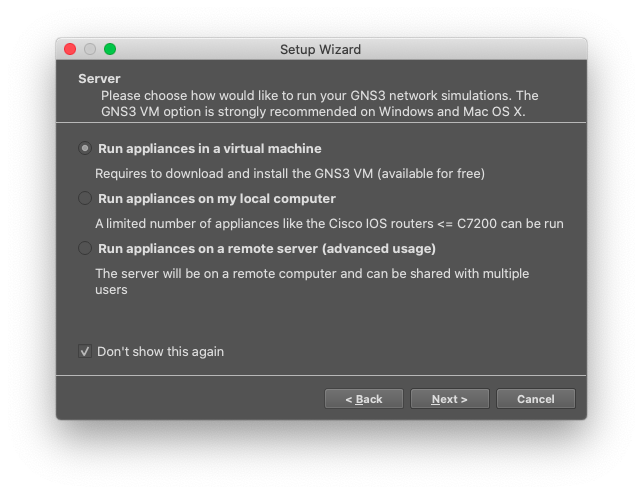
\includegraphics[width=0.8\textwidth]{comparative-gns3-setup-wizard-servers}
  \caption{The GNS3 setup wizard which shows on a fresh installation on by user's demand giving the options running GNS3 distributed}
  \label{fig:comparative-gns3-setup-wizard-servers}
\end{figure}


In GNS3, the lab is running in the server, which, in many cases, is not the user's physical computer.
There is a notion of users connecting to the server (the lab), sharing resources and seeing the effects of actions done by action, which may require some protocols of coordination, e.g. given by the instructor.

\subsection{Portability and sharability of projects}
\label{subsec:comparativeportability}
In texts offering comparisons between network emulators and simulators~\cite{netkit-full,reproduciblenetexp}---in general, software based solutions to replace ``the real thing''---, this is an aspect that has to be taken into account.

On Kathará, if the default Docker images are used (or, in case they are customized, the extended images are published on Docker Hub, and they can always be) the labs are easily shareable and reproducible with the same behavior.

On GNS3, that is not the case.
The dependency
  \begin{enumerate*}[label=(\roman*), itemjoin={{, }}, itemjoin*={{, and }}]
  \item on the proprietary images for either Dynamips or IOSv
  \item in case of using IOSv, on a Linux host for QEMU/KVM support
  \item in case of using Docker nodes as end hosts, which the GNS3's computes can only interact with on Linux hosts, on that operating system
  \end{enumerate*}
as well as the possibility to have distributed labs across more than one server, literally separating the whole set of files needed to reproduce an experiment, and the heavy relying on randomly generated UUIDs, make this more difficult by orders of magnitude. % TODO add UUIDs to acronyms

% end of section comparativenonfunctional


% Section "Performance and resource consumption"
\section{Performance and Resource Consumption}
\label{sec:comparativeperformance}

In terms of resource consumption, experiments with GNS3 and Kathará are very different.
That has an impact in the required computer infrastructures and setups required to do the experiments.
As stated in the explanation between containers-as-lightweight-virtual-machines versus standard \glspl{vm}, a container provides a virtual isolation of the filesystem and networking (among others) for its processes while \glspl{vm} need everything, in every layer of software, a regular host has to run (operating system, libraries, applications) to be loaded each time for each running virtual machine.

In a running Kathará or GNS3 topology, there are associated processes to each node.
As previously shown, GNS3's Cisco routers can be \glspl{vm} running the modern Cisco IOSv or processes of the Dynamips emulator which in fact is a virtual machine, but not in the sense of \textquote{a PC running in isolation with virtualized IO} (e.g. the instructions of those IOS images isn't x86, and therefore there has to be a translation to machine instructions).

Table~\ref{tab:comparativeramusage} lists approximate values measured with the \texttt{top} command (and \texttt{docker~stats}, for Kathará's) on more than one GNU/Linux system for the memory consumption of each process that backs a live node in a topology for each studied possibility.
These measures only approximate the order of magnitude, in a sense that can be described as: \textquote{of several different times the values were measured, on more than one machine, they didn't fluctuate more than, say, $50~\mbox{MiB}$ (for GNS3's) or $5~\mbox{MiB}$ (for Kathará's),} and therefore it doesn't correspond to an accurate arithmetic mean or other formal statistical method.

% Table tab:comparativeramusage
\begin{table}
  \centering
  \small
  \begin{tabulary}{0.9\textwidth}{ll}
    \toprule
      \textbf{Topology node}                   & \textbf{Memory usage}\\
    \midrule
      GNS3 -- Cisco IOSvL2 (KVM via QEMU)      & $\approx 460~\mbox{MiB}$\\
      GNS3 -- Cisco c3745 (Dynamips process)   & $\approx 270~\mbox{MiB}$\\
      Kathará (any node is a Docker container) & $\approx 4~\mbox{MiB}$\\
    \bottomrule
  \end{tabulary}
  \caption{%
    Approximate metrics of the memory footprint of (networking) nodes in topologies for different emulators
  }
  \label{tab:comparativeramusage}
\end{table}


For the sake of example, the query for the memory footprint of the running Docker containers on a host (in this case, all of them are Quagga-enabled Linux hosts as Kathará nodes) is shown in figure~\ref{fig:comparative-docker-stats}.

% Figure fig:comparative-docker-stats
\begin{figure}
  \centering
  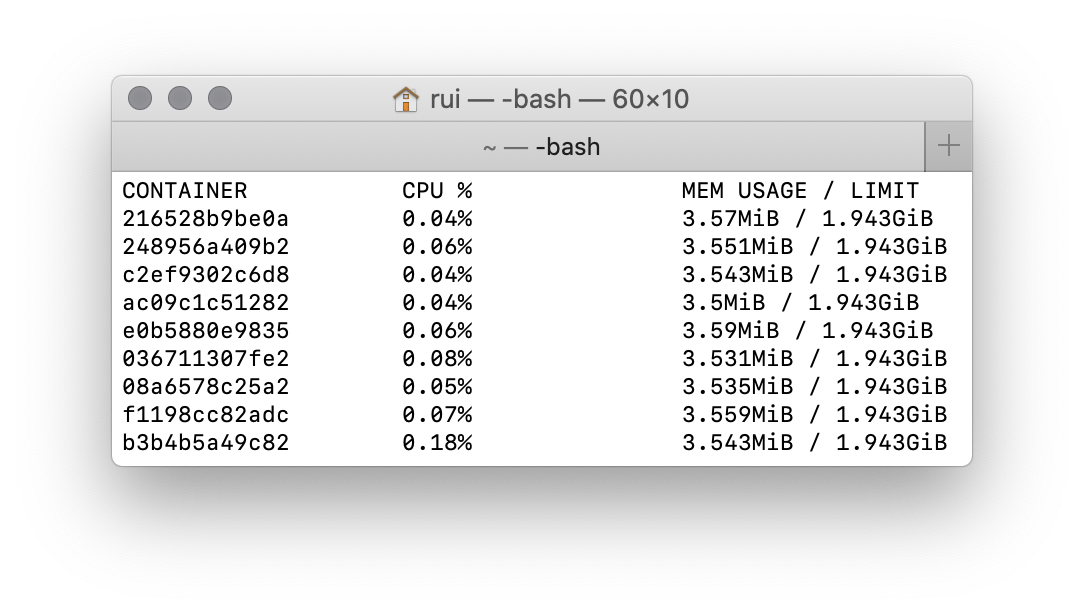
\includegraphics[width=0.8\textwidth]{comparative-docker-stats}
  \caption{The \texttt{docker stats} command showing the resources taken by containers corresponding to nodes in a Kathará lab}
  \label{fig:comparative-docker-stats}
\end{figure}


% end of section comparativeperformance


% end of chapter

  % % !TEX root = ../Thesis.tex
% !TEX spellcheck = en-US

\chapter{Conclusions and further work}
\label{ch:conclusions}

In this chapter, our provisional conclusions, we're not doing nothing else than using a term in the glossary to force it to be printed.
We have decided that term to be~\gls{Real numbers}.

With this, we conclude this long document.
Thank you for reading!

% \section{Section 1}
% \label{sec:relsec1}

% \section{Section 2}
% \label{sec:relsec2}

% end of chapter


% This ensures that the subsequent sections are being included as root
% items in the bookmark structure of your PDF reader.
% \bookmarksetup{startatroot}
% \backmatter

%   \begingroup
%     \let\clearpage\relax
%     \glsaddall
%     \printglossary[type=\acronymtype]
%     \newpage
%     \printglossary
%   \endgroup

  \printindex
  \printbibliography

\end{document}

% \begin{document}
% \frontmatter

% \maketitle

% \tableofcontents

% % Introductory chapters
% \chapter{Preface}
% % ...

% \mainmatter
% \chapter{First chapter}
% % ...

% \appendix
% \chapter{First Appendix}

% \backmatter
% \chapter{Last note}
% \end{document}
